\documentclass[13pt]{beamer}
% \usecolortheme{whale}
\usetheme{Boadilla}
\usecolortheme{seahorse}
% \usetheme{Singapore}
\usepackage{lipsum}
\usepackage{fancybox}
% \usepackage{fontspec}
\usepackage{xeCJK}
\setCJKmainfont[AutoFakeBold=true]{TW-Sung}
% \setCJKsansfont{Kurier}

\setbeamertemplate{navigation symbols}{}

\usepackage{tabto}
\usepackage{parskip}  % No-indent
% \usepackage{enumitem} % change enumerate behaviours
\usepackage{lipsum} %
\usepackage{color}
\usepackage{siunitx}
\usepackage{newclude} %make include only not clearpage
\usepackage{multicol}
\setlength{\fboxsep}{0.6em}
\usepackage{graphics}
\usepackage{tabularx}
\usepackage{tcolorbox}
\usepackage{makecell}
\usepackage{tikz}
\usetikzlibrary{positioning}
\usepackage{tasks}
\input{mcmacro}






%Information to be included in the title page:
\title{第二課}
\author{波的現象}
\institute{全年班}
\date{}

% \setbeamerfont{normal text}{size=\HUGE}
% \setbeamerfont{block title}{size=\HUGE}

\newcounter{saveenumi}
\newcommand{\seti}{\setcounter{saveenumi}{\value{enumi}}}
\newcommand{\conti}{\setcounter{enumi}{\value{saveenumi}}}


\newcommand{\shc}[1]{
    \qty[mode = text]{#1}{J.kg^{-1}.\degreeCelsius^{-1}}
}
\newcommand{\hc}[1]{
    \qty[mode = text]{#1}{J.\degreeCelsius^{-1}}
}
\newcommand{\oc}[1]{
\qty{#1}{\degreeCelsius}
}
\newcommand{\slh}[1]{\qty{#1}{J.kg^{-1}}}

\newcommand{\dg}[1]{ \qty{#1}{^{\circ}} }


\begin{document}
\frame{\titlepage}

\begin{frame}{連續機械行波的能量分佈}
    \begin{block}{考慮某一瞬間各質點的能量/單一質點隨時間推移的能量:}
        \begin{itemize}
            \item 質點的總機械能=動能+勢能
                  \begin{itemize}
                      \item 總機械能:跟振幅相關。
                      \item 勢能:跟位移相關。
                      \item 動能:跟質點的移動速率相關。
                  \end{itemize}
            \item 若沒有能量損耗,總機械能不變。
        \end{itemize}
    \end{block}





\end{frame}


\begin{frame}{連續機械行波的能量分佈}
    \begin{figure}
        \centering
        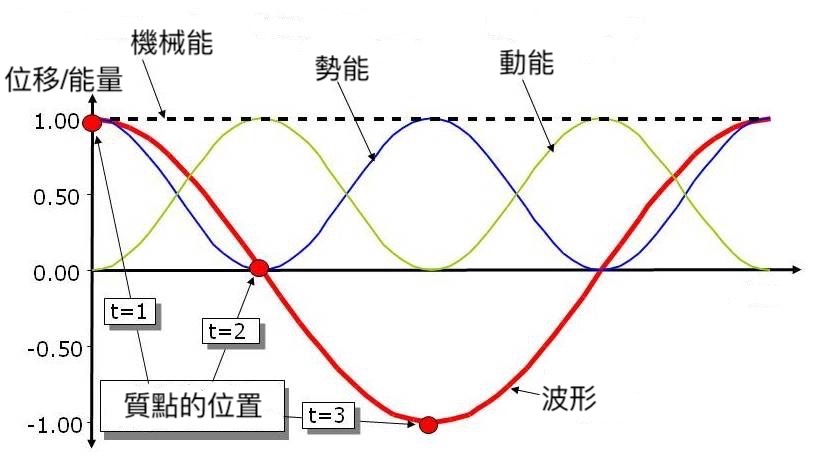
\includegraphics[width=1\linewidth]{images/231.pic4.jpg}


    \end{figure}
\end{frame}

\begin{frame}{}
    圖(a)顯示九個均勻分佈的質點。圖(b)顯示一縱波各質點的位置。在此時此刻,下列哪線圖正確地顯示各點的勢能PE隨位置x的變化?
    \begin{figure}
        \centering
        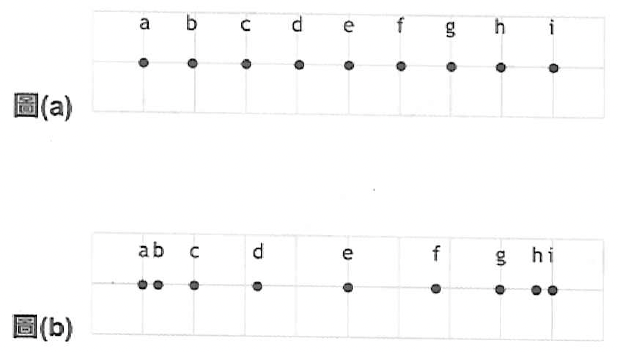
\includegraphics[width=0.5\linewidth]{images/Screenshot 2023-09-27 at 8.21.03 AM.png}


    \end{figure}
    \begin{mmchoices}
        \item \topalign{
            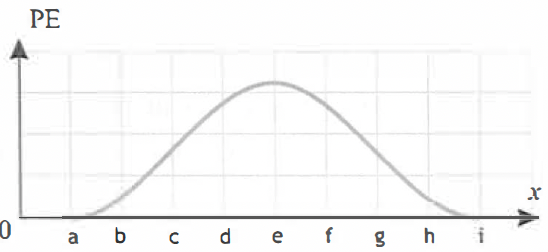
\includegraphics[width=0.75\linewidth]{images/Screenshot 2023-09-27 at 8.30.49 AM.png}

        }
        \item \topalign{    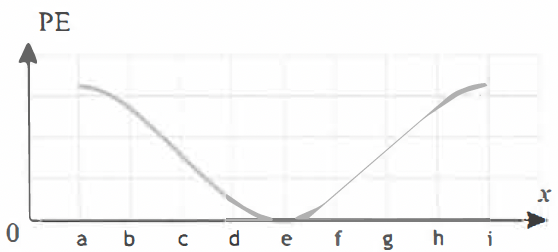
\includegraphics[width=0.75\linewidth]{images/Screenshot 2023-09-27 at 8.30.55 AM.png}
        }
        \item \topalign{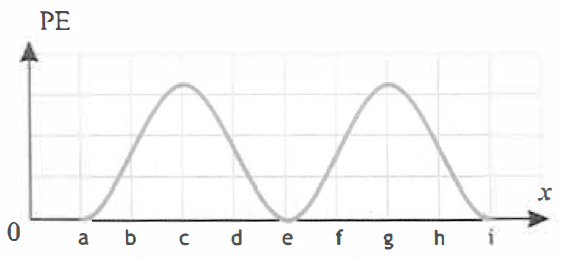
\includegraphics[width=0.75\linewidth]{images/Screenshot 2023-09-27 at 8.31.00 AM.png}}

        \item \topalign{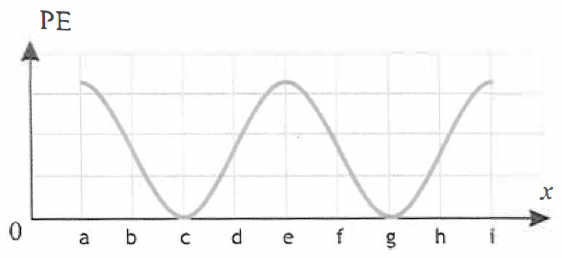
\includegraphics[width=0.75\linewidth]{images/Screenshot 2023-09-27 at 8.31.03 AM.png}}

    \end{mmchoices}
\end{frame}




\begin{frame}{水波槽}

    \begin{figure}
        \centering
        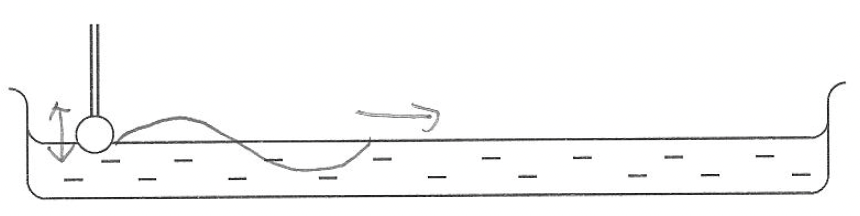
\includegraphics[width=0.5\linewidth]{images/Screenshot 2023-09-25 at 2.25.17 AM.png}
        % 
    \end{figure}
    \begin{figure}
        \centering
        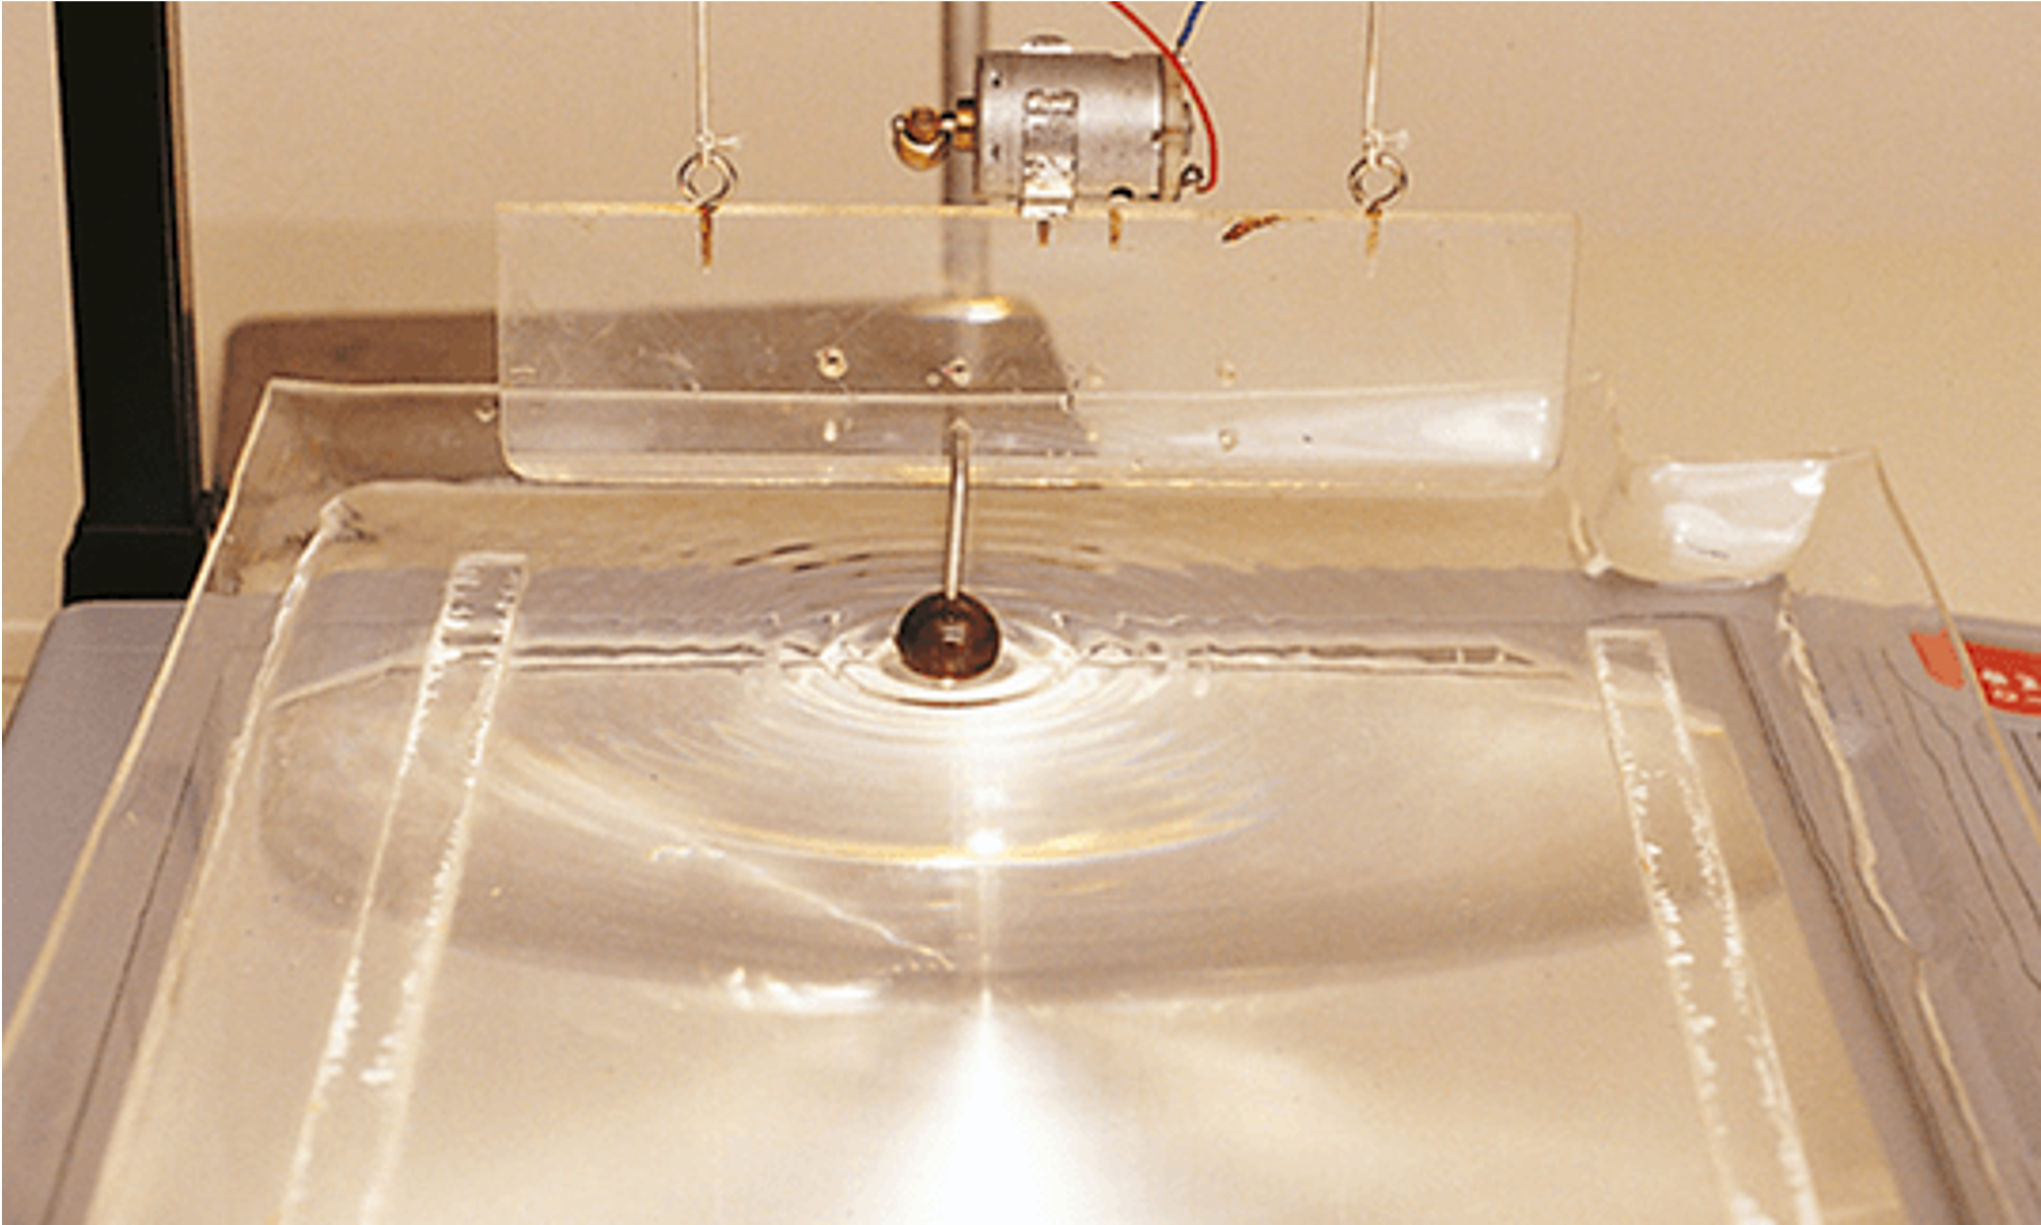
\includegraphics[width=0.5\linewidth]{images/Picture 1.png}
        \caption{水波槽可以用來產生水波}

    \end{figure}
\end{frame}




\begin{frame}{水波的前進}
    \begin{itemize}
        \item 當點振源移動一次上下一個完整的周期時,會產生一個完整的水波波長。\begin{itemize}
                  \item 點振源的頻率=水波的頻率。
                  \item 點振源無法控制水波的速率。
                  \item $v=f\ \lambda$,頻率越大,波長越短。
              \end{itemize}
    \end{itemize}
    \begin{figure}
        \centering
        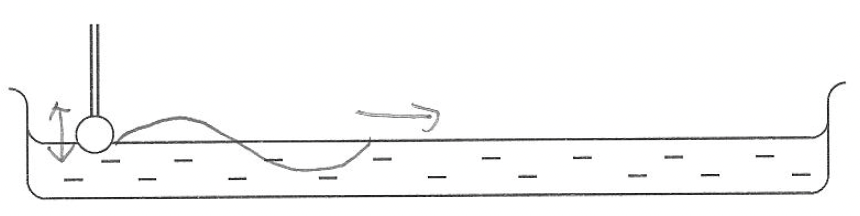
\includegraphics[width=0.5\linewidth]{images/Screenshot 2023-09-25 at 2.25.17 AM.png}
        % \caption{水波槽可以用來}
    \end{figure}
\end{frame}

\begin{frame}{製造水波}
    \begin{columns}
        \column{.5\textwidth}
        \begin{figure}
            \centering
            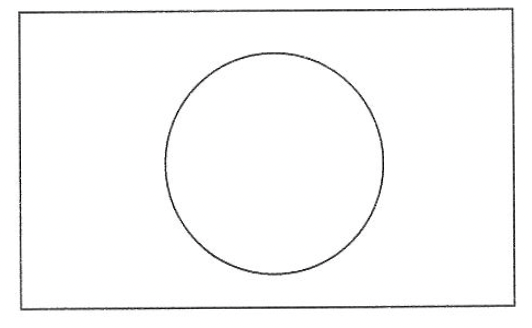
\includegraphics[width=0.97\linewidth]{images/Screenshot 2023-09-25 at 2.30.30 AM.png}
            \caption{脈衝水波}

        \end{figure}
        \column{.5\textwidth}
        \begin{figure}
            \centering
            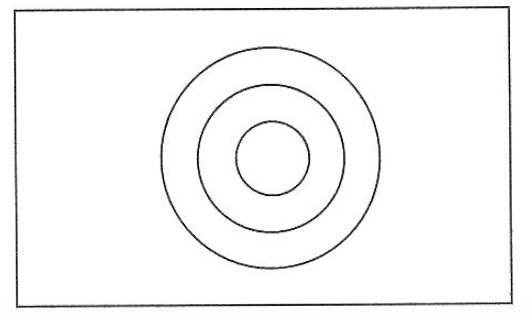
\includegraphics[width=1\linewidth]{images/Screenshot 2023-09-25 at 2.31.45 AM.png}
            \caption{連續水波}

        \end{figure}
    \end{columns}
\end{frame}



\begin{frame}{以不同角度觀察水波}
    \begin{figure}
        \centering
        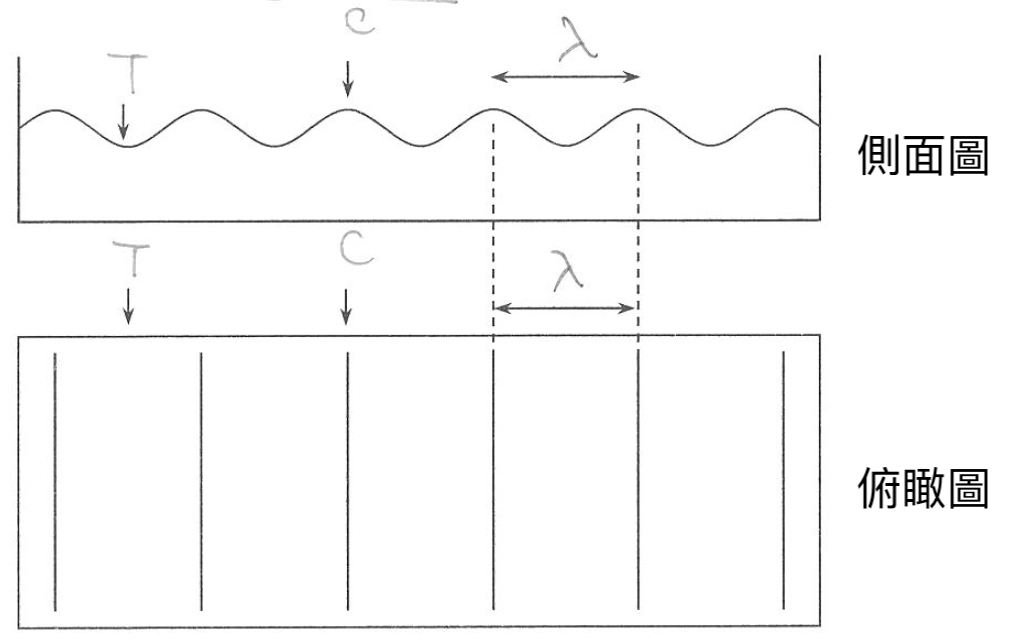
\includegraphics[width=1\linewidth]{images/Screenshot 2023-09-25 at 2.33.31 AM.png}


    \end{figure}
\end{frame}


\begin{frame}{在屏幕上形成的條紋}
    \begin{figure}
        \centering
        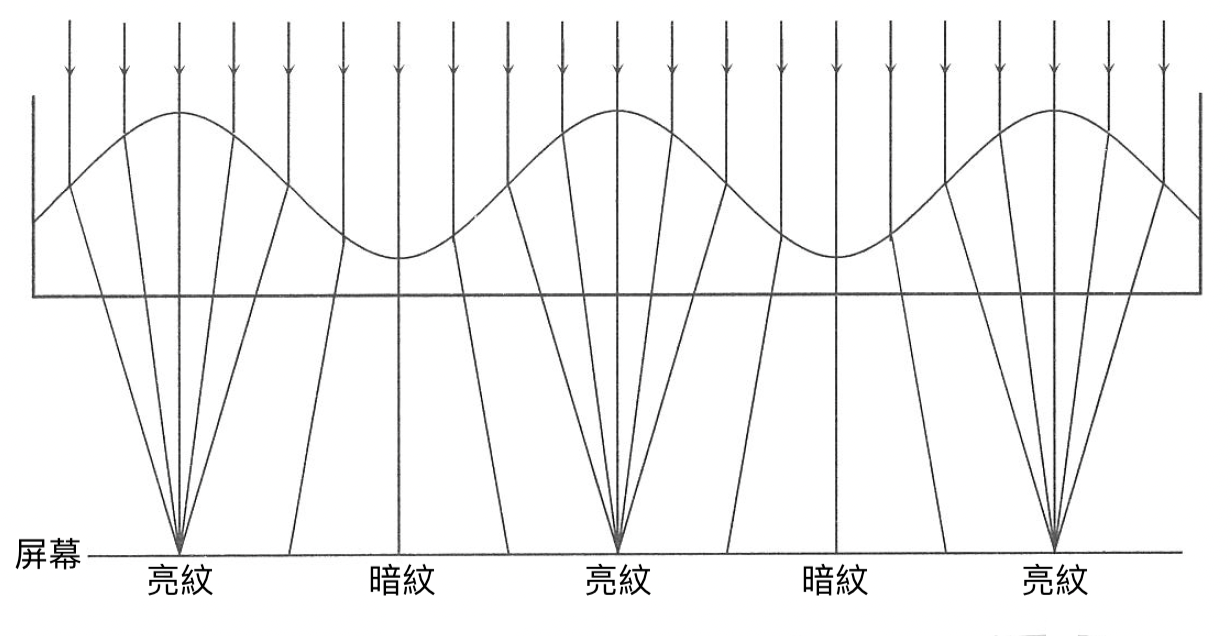
\includegraphics[width=0.75\linewidth]{images/Screenshot 2023-09-26 at 9.55.36 PM.png}
    \end{figure}
    \begin{itemize}
        \item 波峰聚焦光線形成光紋。
        \item 波谷發散光線形成暗紋。
    \end{itemize}
\end{frame}


\begin{frame}{波陣面和射線}
    \begin{itemize}
        \item 波峰連接的線稱為波陣面。
        \item 在同一波陣面上,所有質點都以同相振動。
        \item 射線:表示波的傳播方向的線
        \item 波陣面必定垂直於射線。
    \end{itemize}\bigskip
    \begin{columns}
        \column{.5\textwidth}
        \begin{figure}
            \centering
            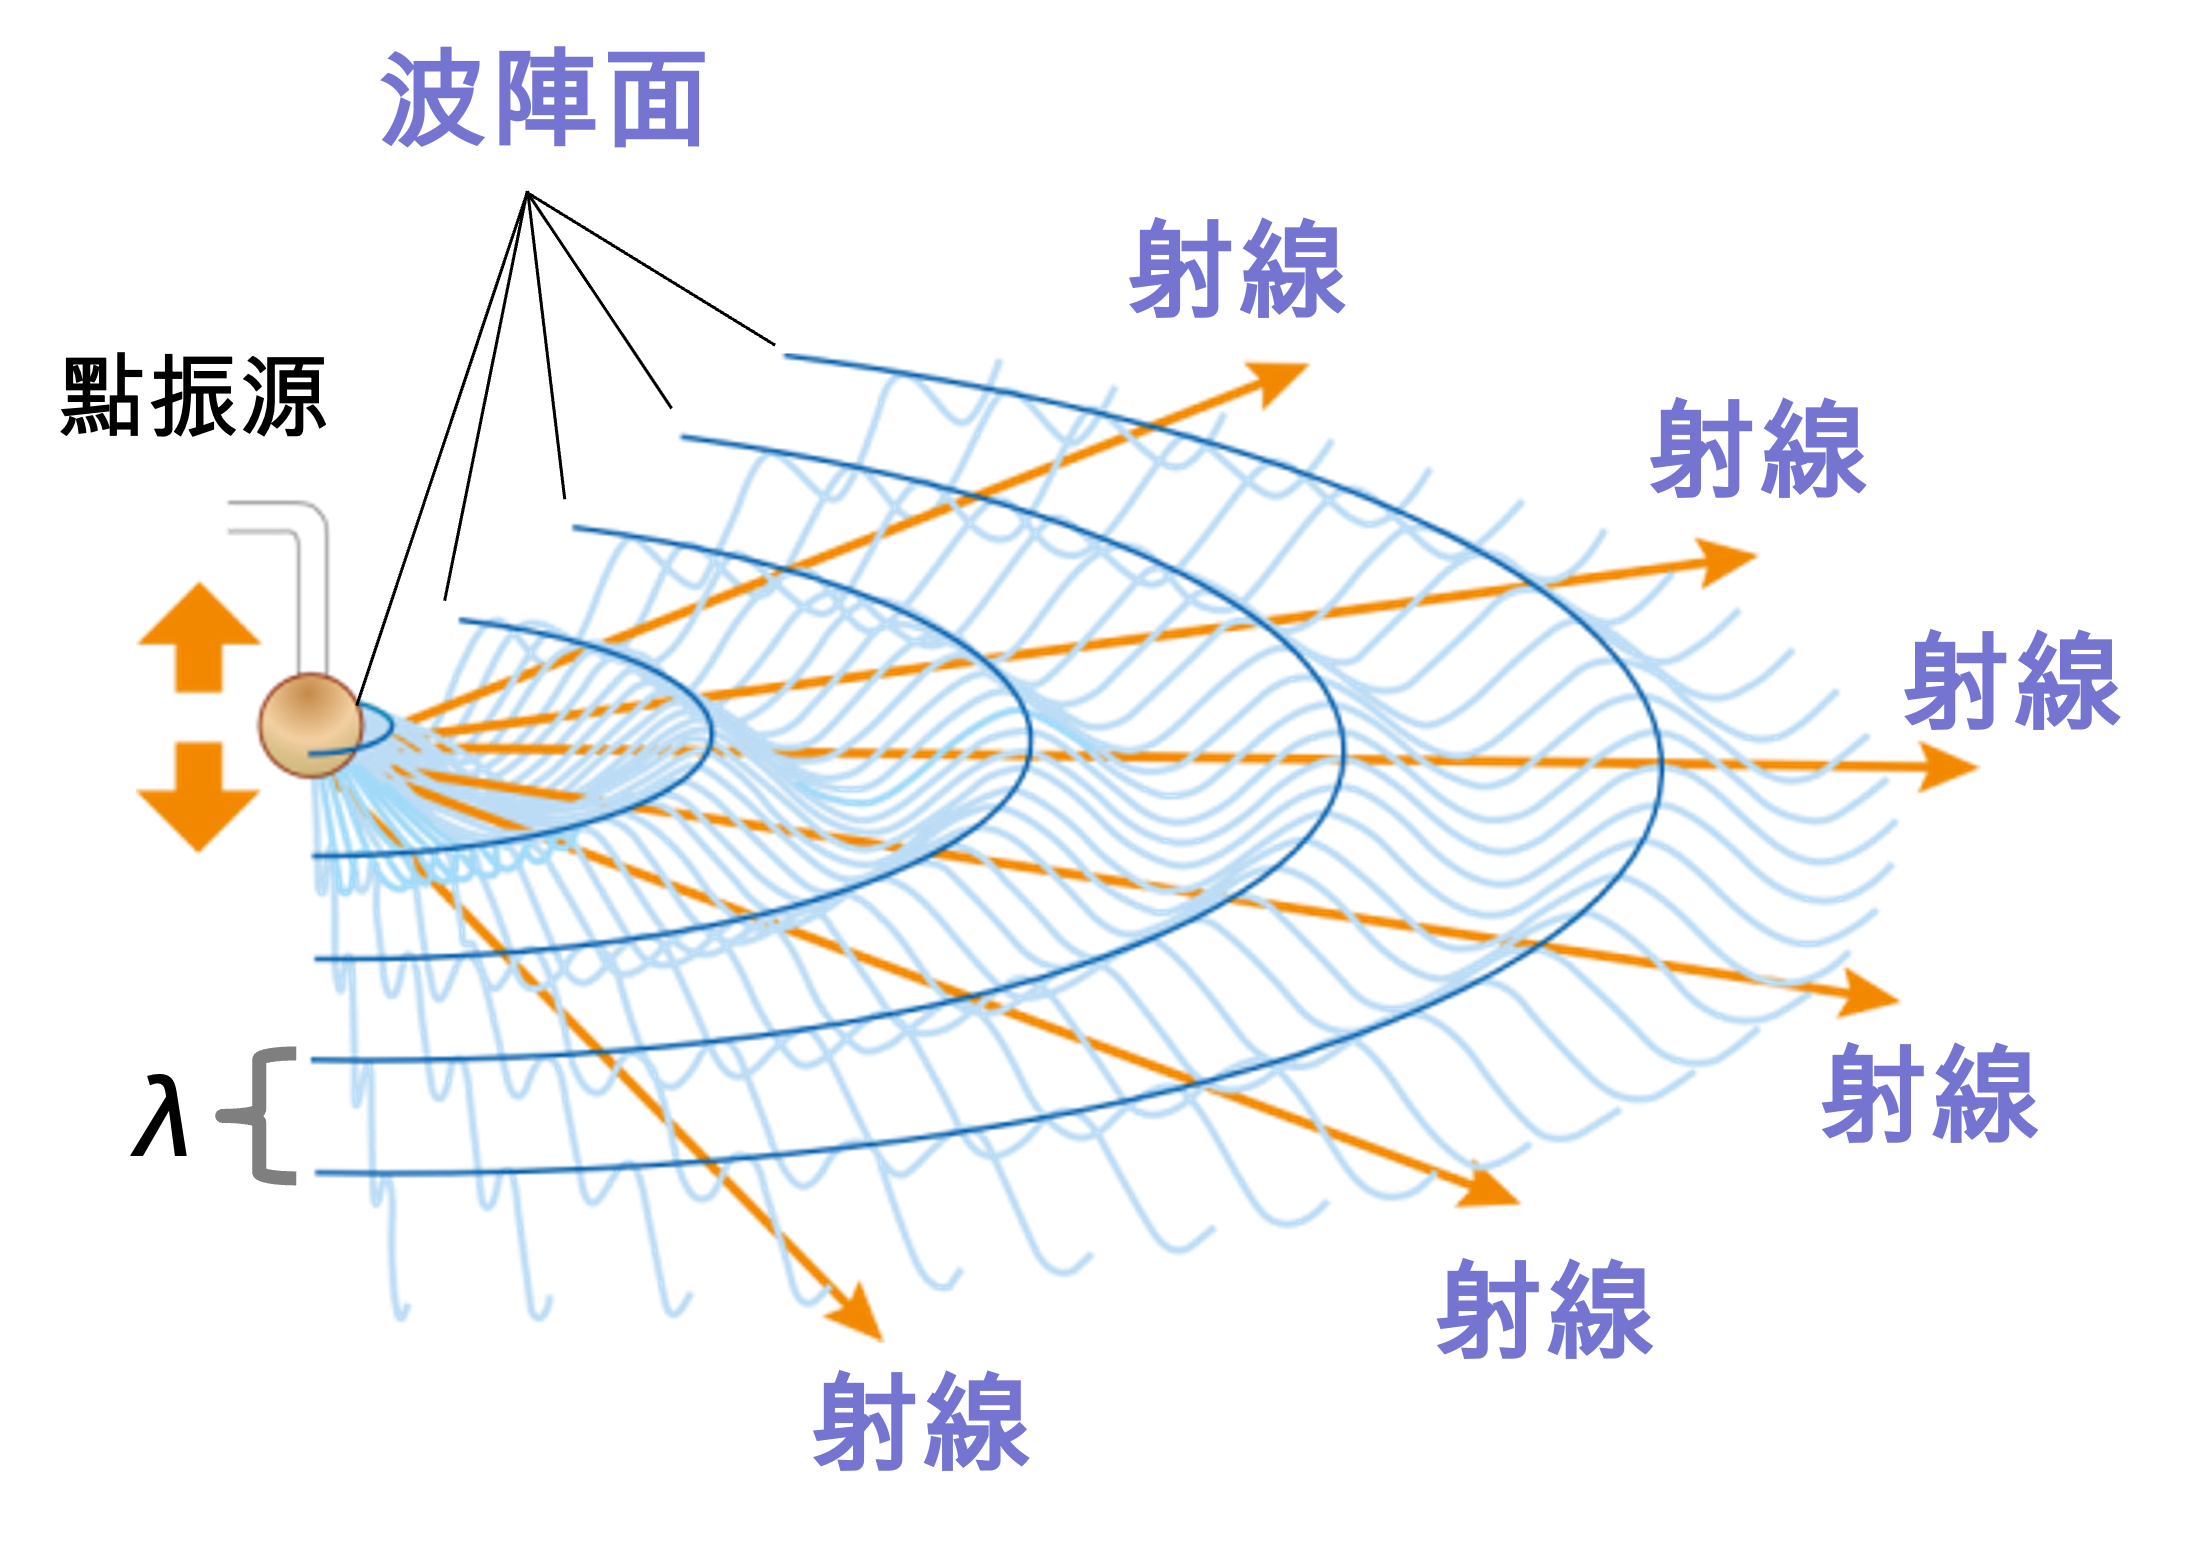
\includegraphics[width=\linewidth]{images/1}
            % \caption{點振源產生圓形波陣面}

        \end{figure}

        \column{.5\textwidth}
        % \begin{figure}
        %     \centering
        %     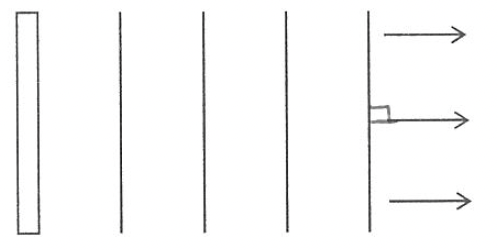
\includegraphics[width=1\linewidth]{images/Screenshot 2023-09-25 at 2.39.25 AM.png}
        %     \caption{直振源產生直線波陣面}

        % \end{figure}
        \begin{figure}
            \centering
            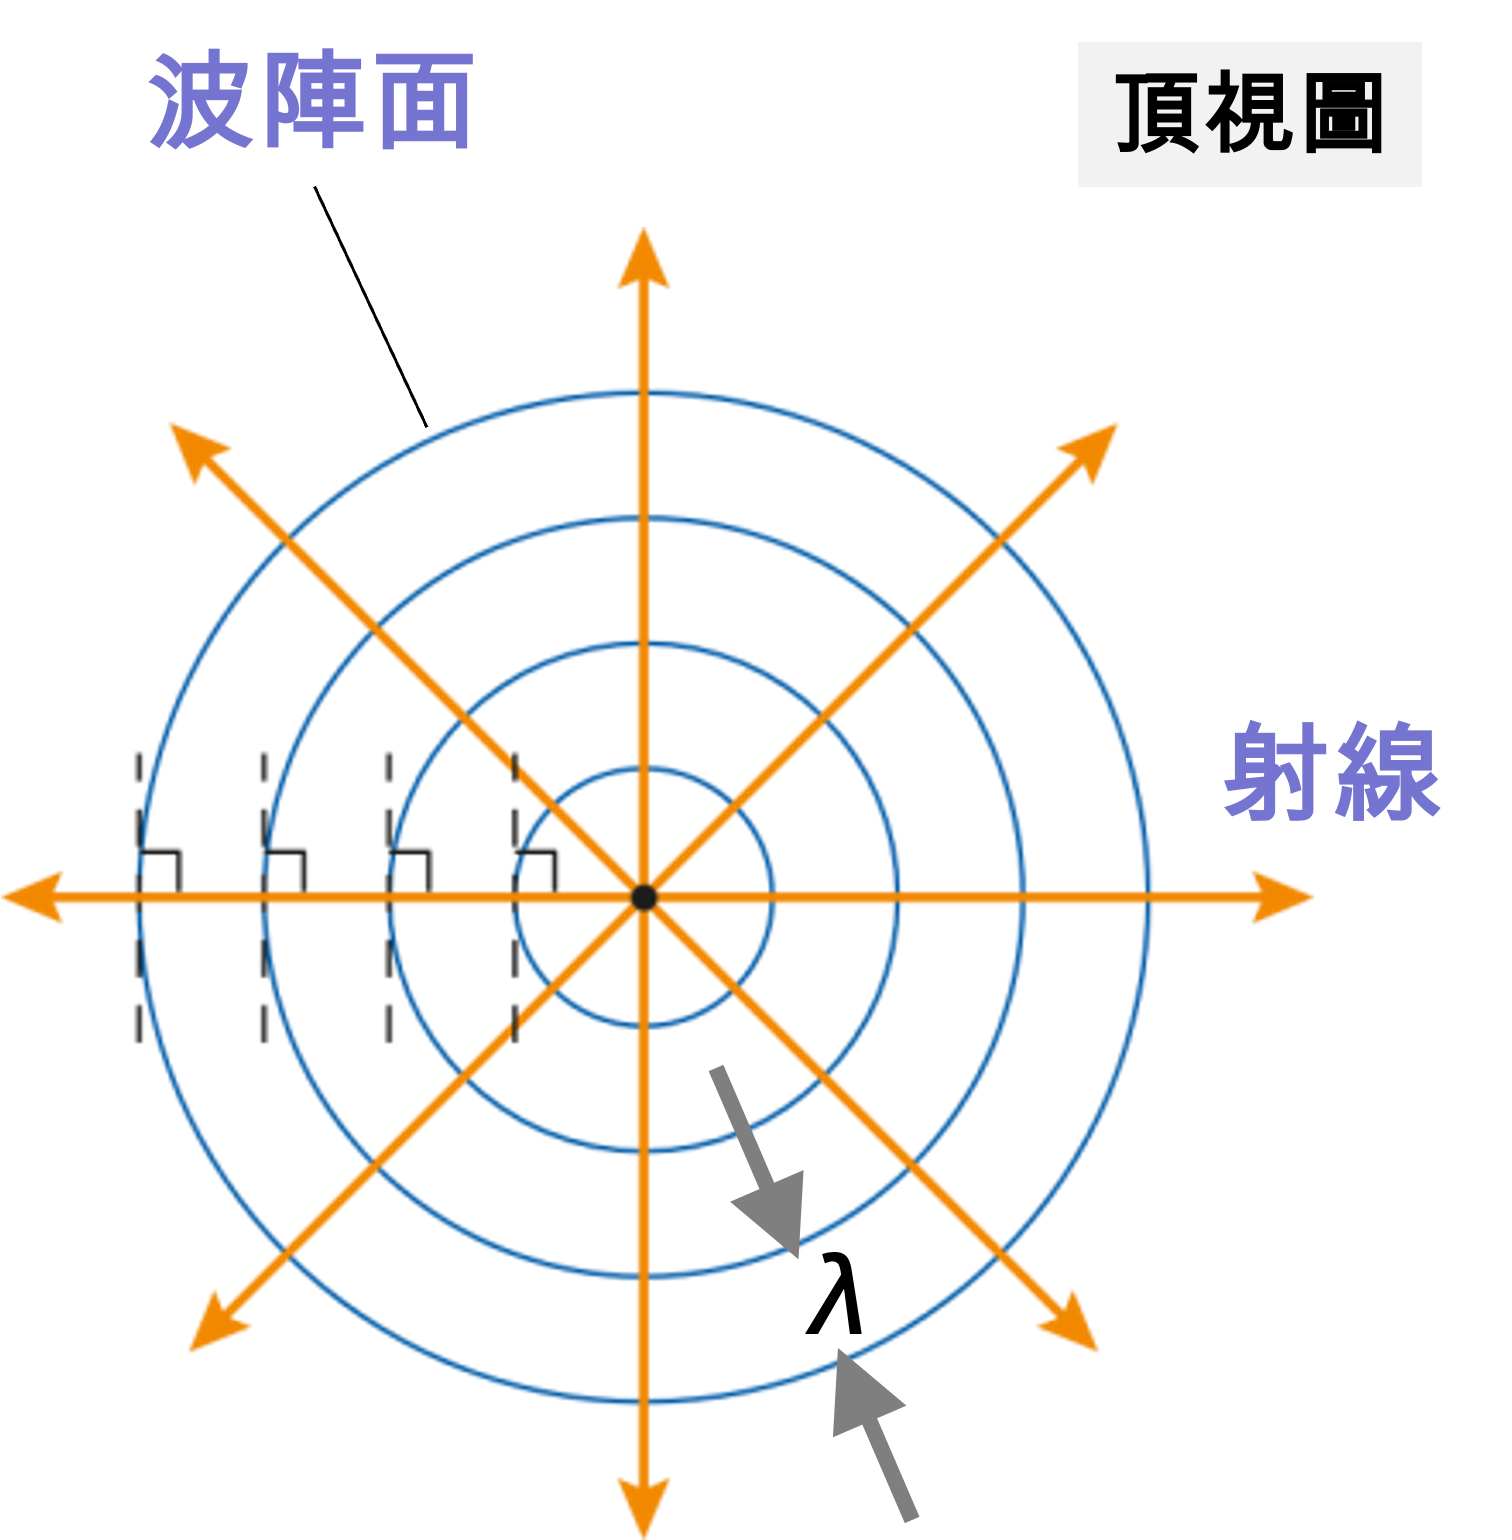
\includegraphics[width=0.7\linewidth]{images/2.png}
            % \caption{點振源產生圓形波陣面}

        \end{figure}
        % \begin{figure}
        %     \centering
        %     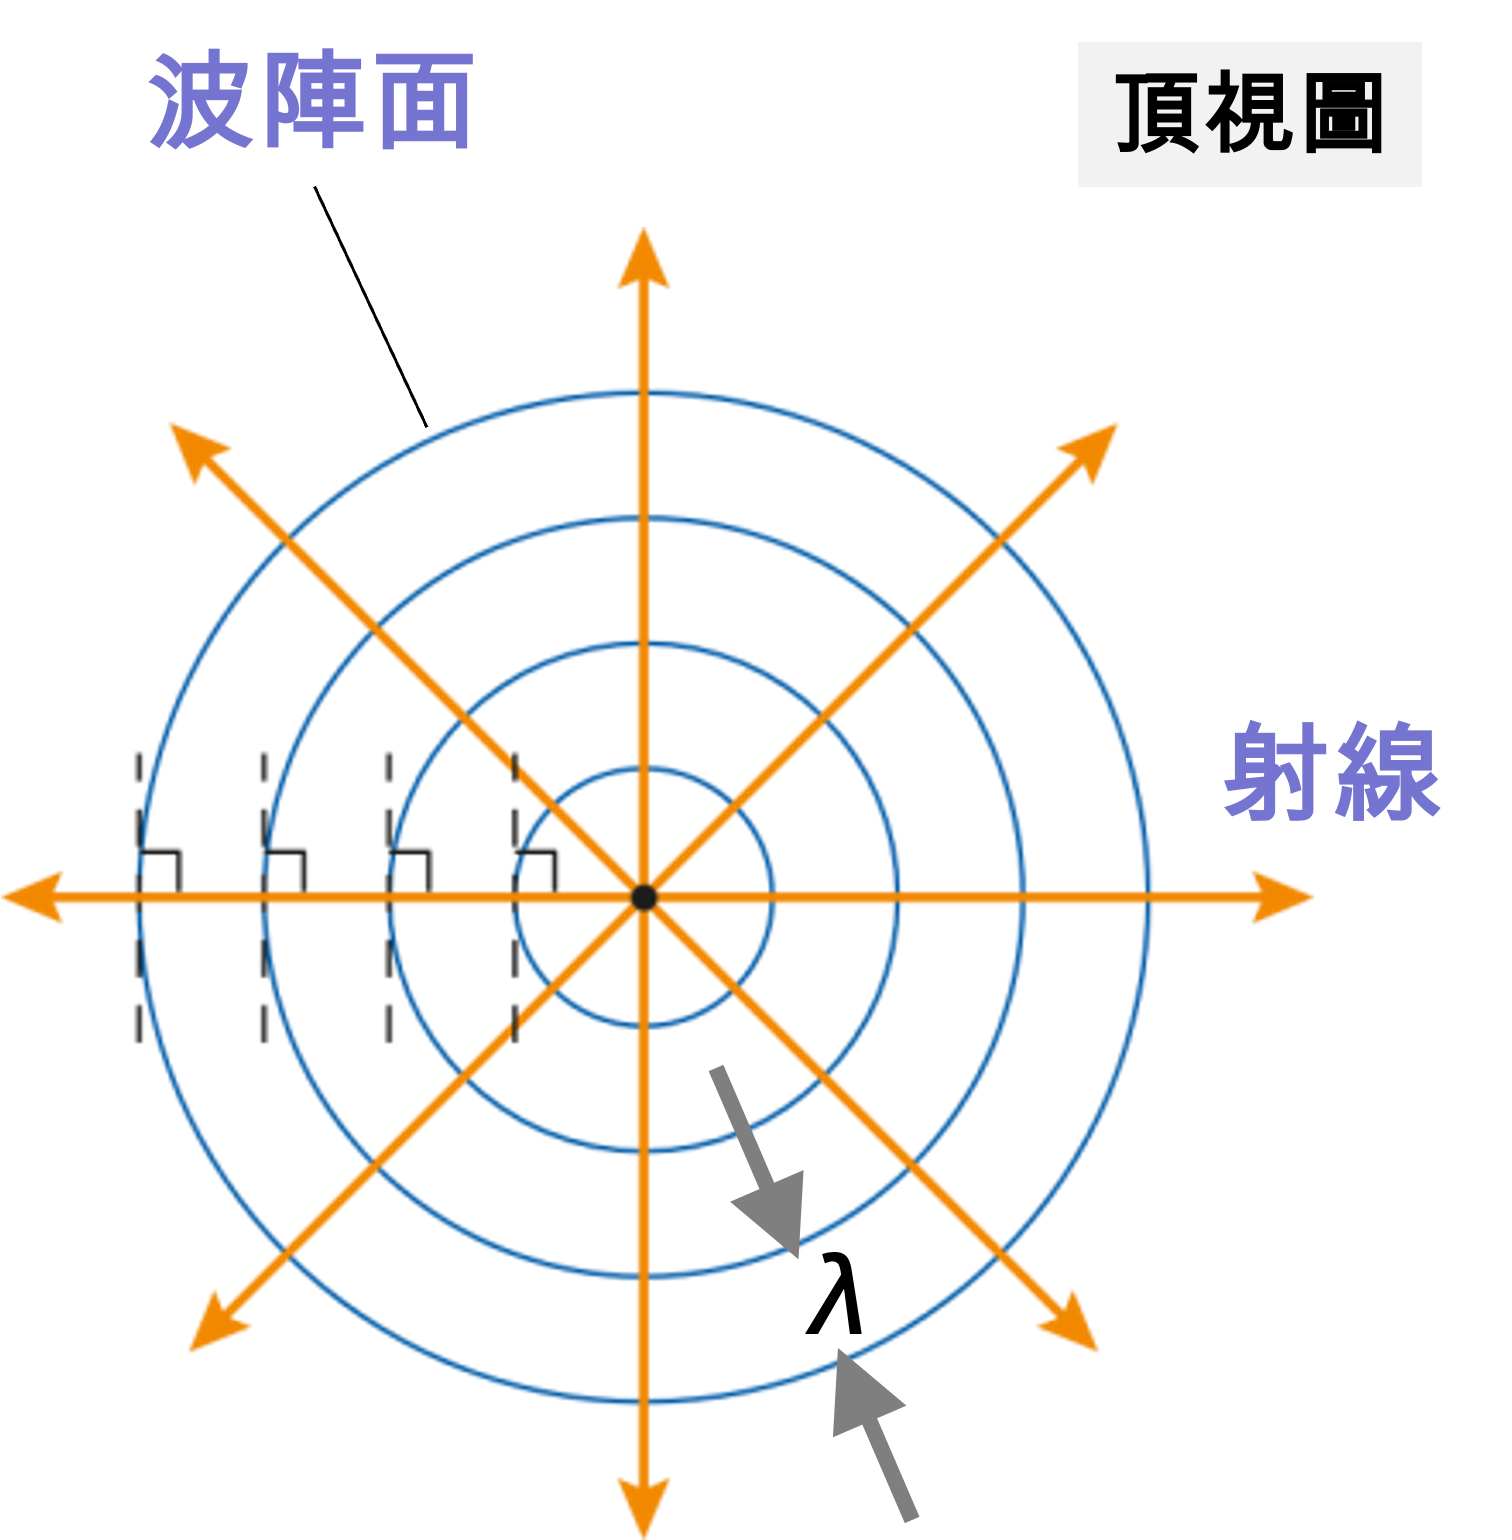
\includegraphics[width=1\linewidth]{images/2.png}


        % \end{figure}
    \end{columns}
\end{frame}

\begin{frame}{波陣面和射線}
    \begin{columns}
        \column{.5\textwidth}
        \begin{figure}
            \centering
            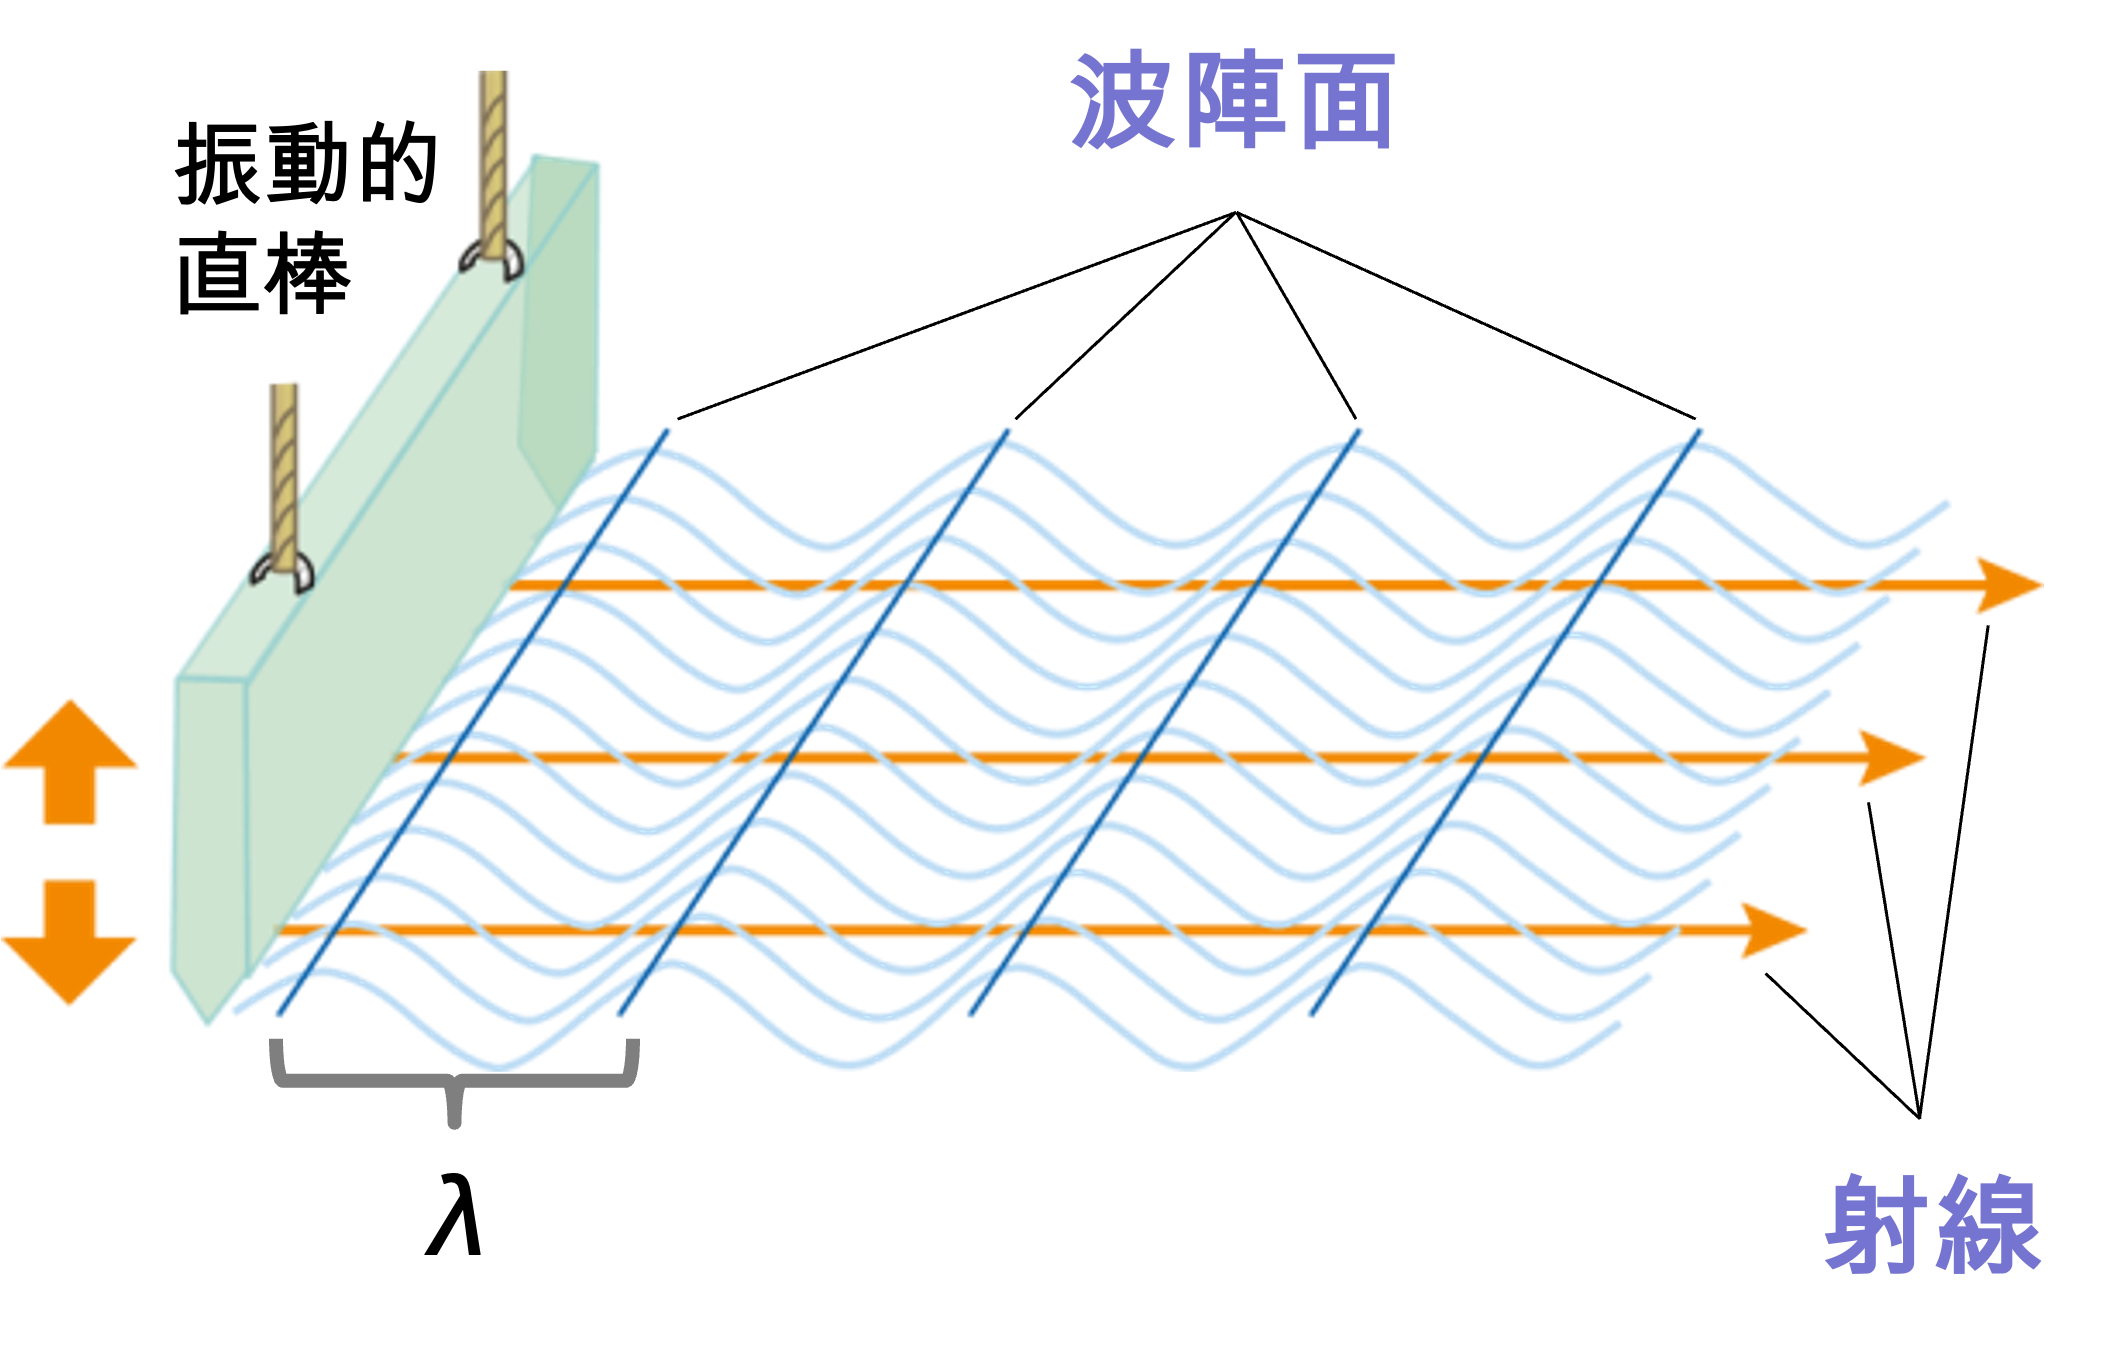
\includegraphics[width=1\linewidth]{images/3.png}


        \end{figure}
        \column{.5\textwidth}
        % \begin{figure}
        %     \centering
        %     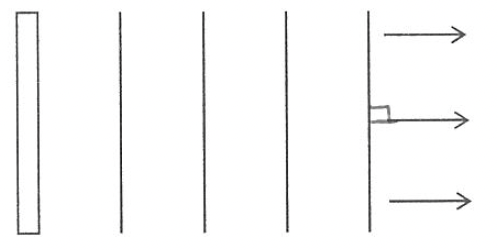
\includegraphics[width=1\linewidth]{images/Screenshot 2023-09-25 at 2.39.25 AM.png}
        %     \caption{直振源產生直線波陣面}

        % \end{figure}
        \begin{figure}
            \centering
            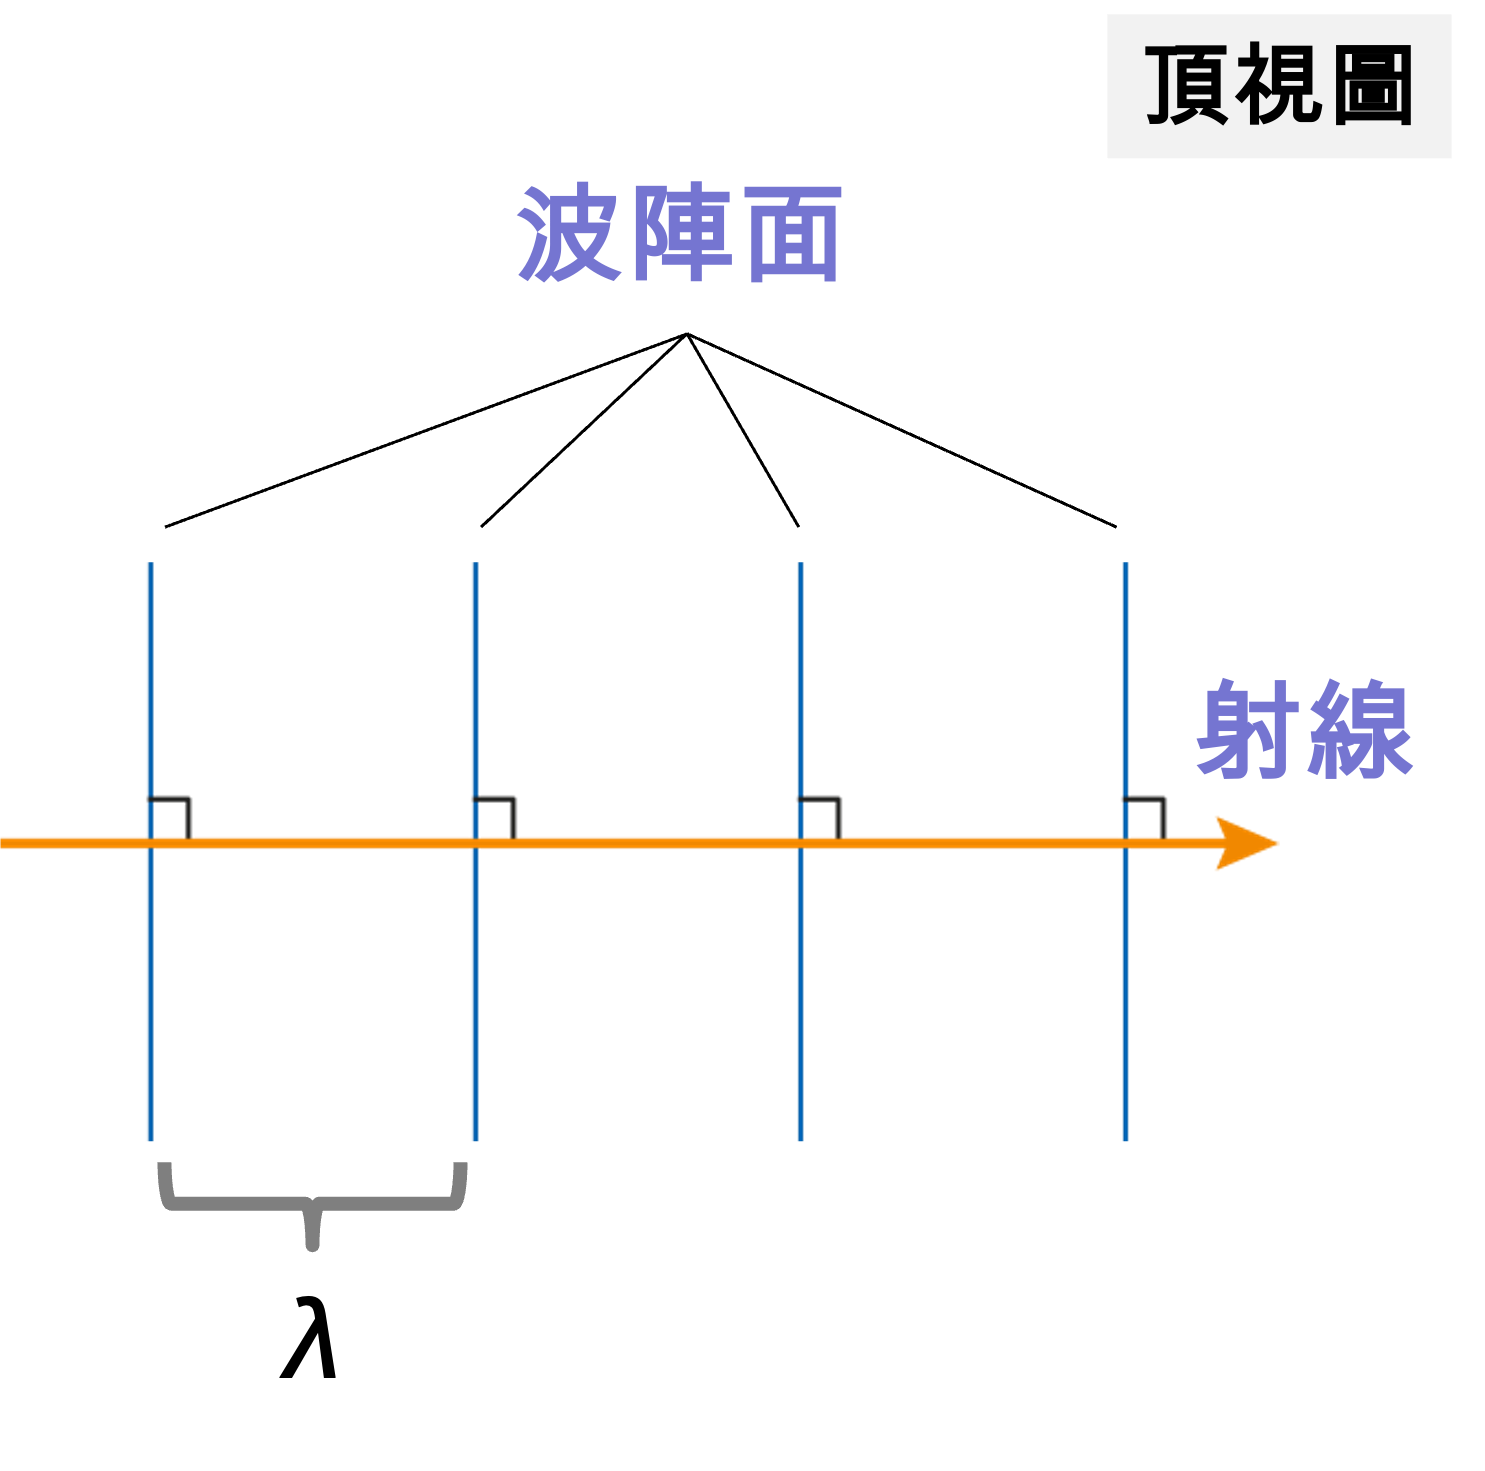
\includegraphics[width=1\linewidth]{images/4.png}


        \end{figure}
        % \begin{figure}
        %     \centering
        %     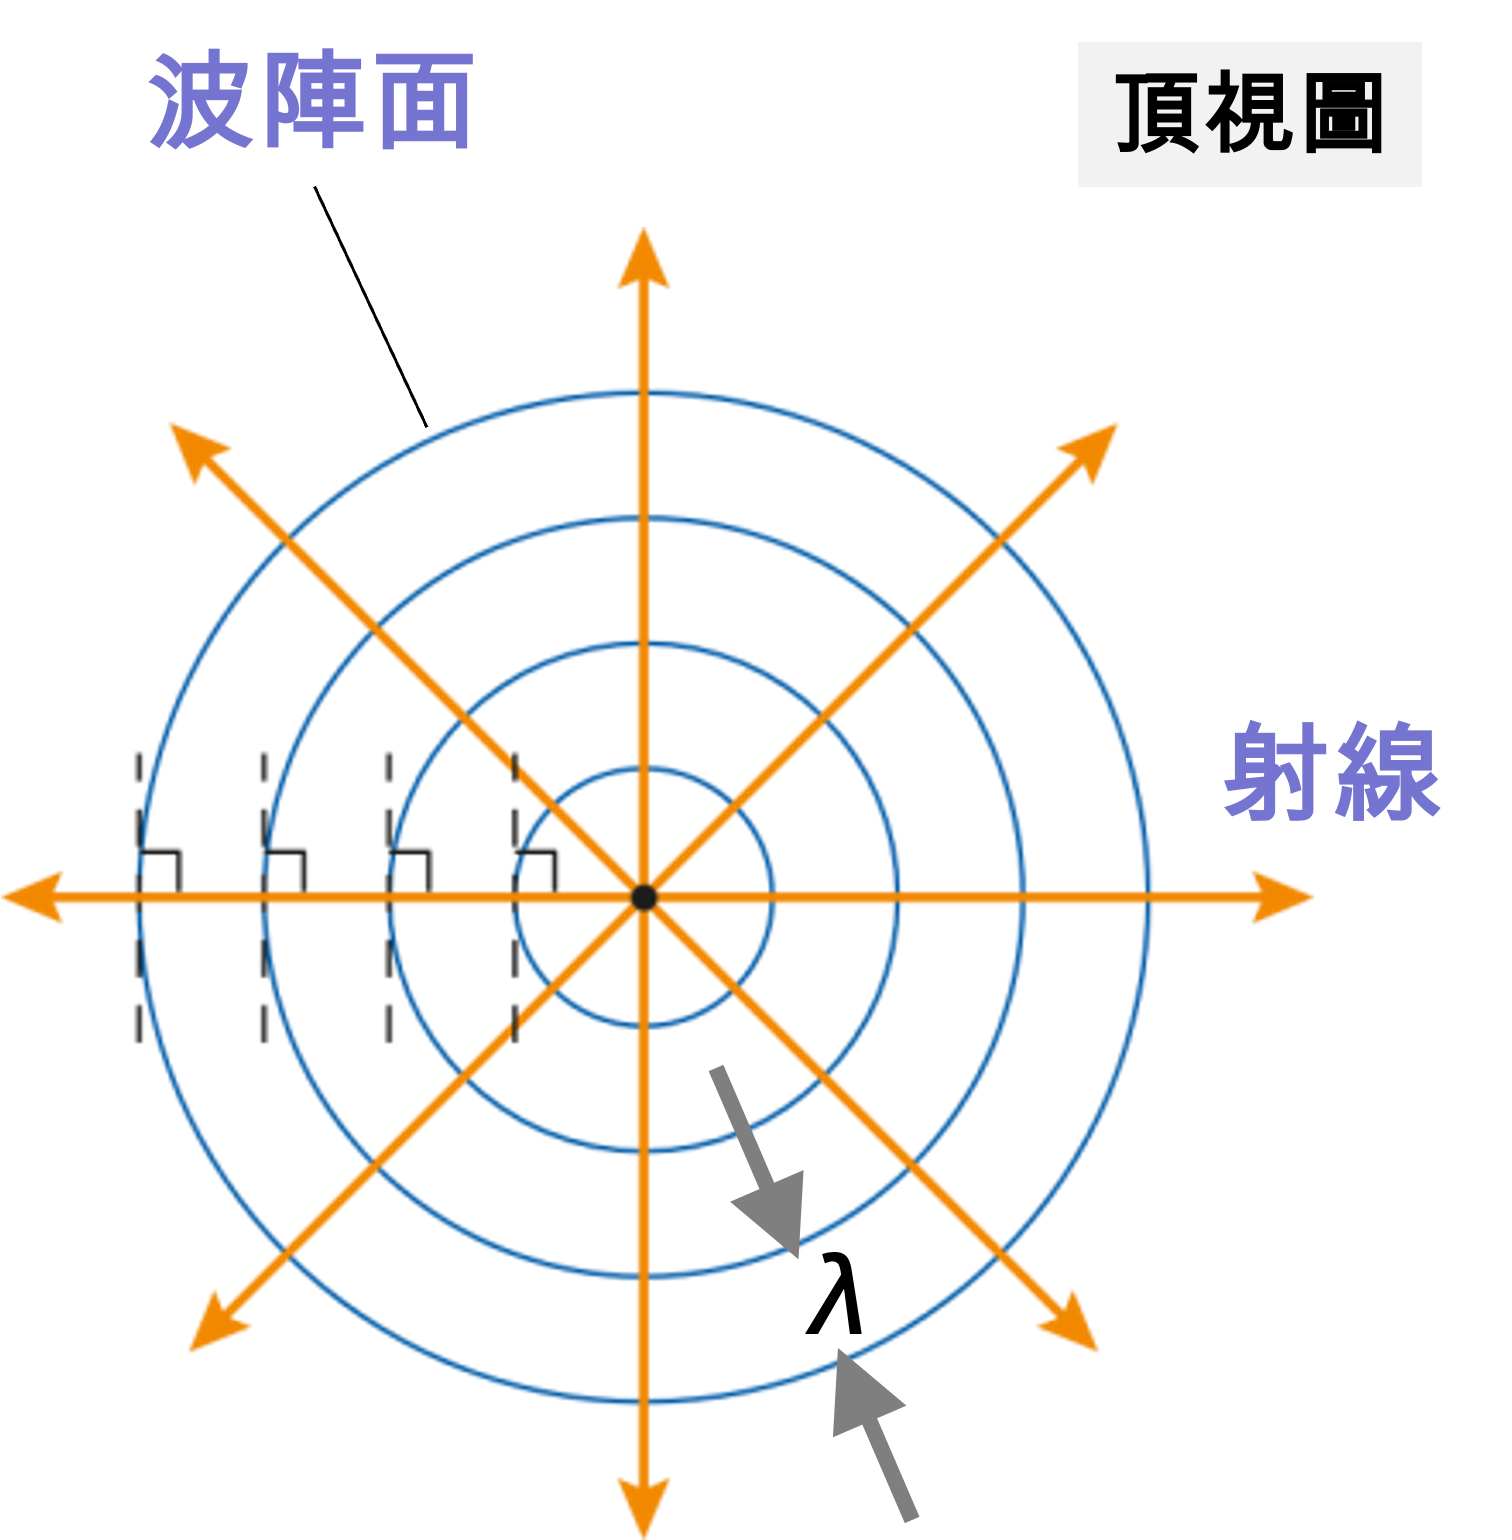
\includegraphics[width=1\linewidth]{images/2.png}


        % \end{figure}
    \end{columns}
\end{frame}

\begin{frame}[t]{例題}
    左圖和右圖分別是兩個直線水波P和Q。其中P的水比較淺。比較兩波的\(\lambda,v,f\)。
    \begin{figure}
        \centering
        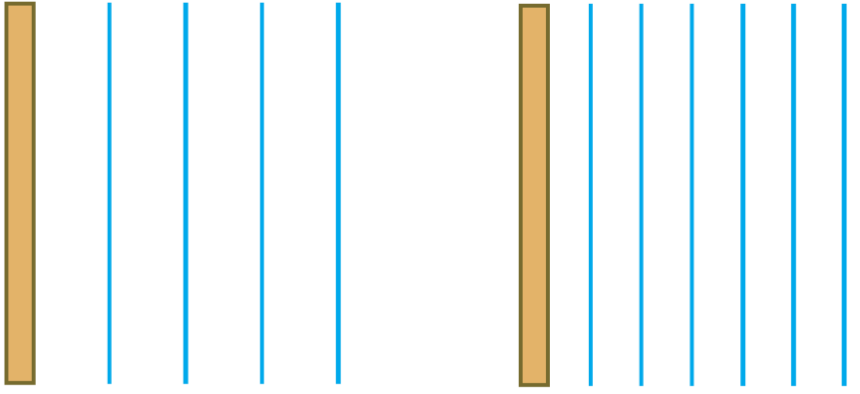
\includegraphics[width=0.65\linewidth]{images/Screenshot 2023-09-26 at 11.25.42 PM.png}


    \end{figure}
\end{frame}

\begin{frame}{量度水波的頻率}
    \begin{itemize}
        \item 在黑暗的環境下,調整頻閃觀察器的頻率直至波形看起來靜止不動。
        \item 這時頻閃觀察器的頻率=波的頻率。
    \end{itemize}\bigskip
    \begin{columns}
        \column{.5\textwidth}
        \begin{figure}
            \centering
            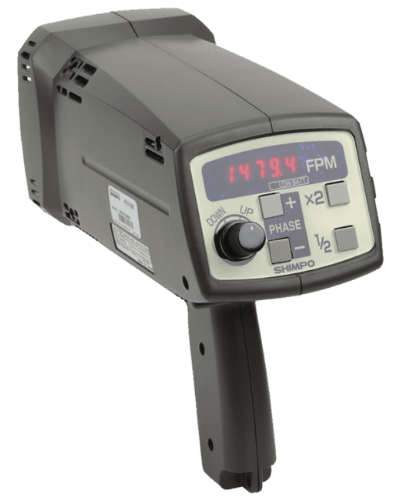
\includegraphics[width=0.6\linewidth]{images/Screenshot 2023-09-26 at 10.05.09 PM.png}


        \end{figure}
        \column{.5\textwidth}
        \begin{figure}
            \centering
            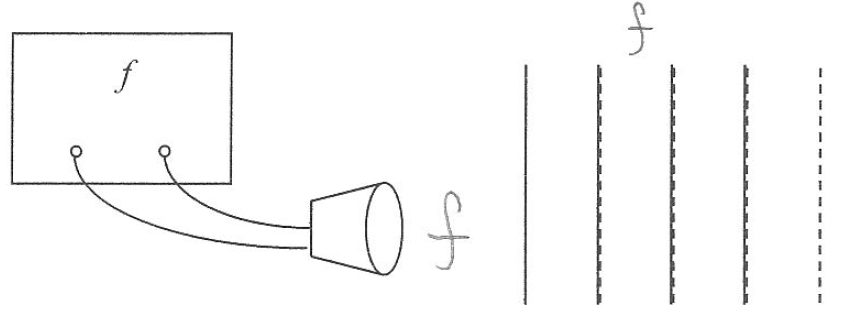
\includegraphics[width=1\linewidth]{images/Screenshot 2023-09-26 at 10.08.47 PM.png}


        \end{figure}
    \end{columns}
\end{frame}
\begin{frame}{量度水波的波長}
    \begin{itemize}
        \item 調整頻閃觀察器的頻率直至波形看起來靜止不動。
        \item 使用米尺量度幾個連續水波的波長。
    \end{itemize}\bigskip
    \begin{figure}
        \centering
        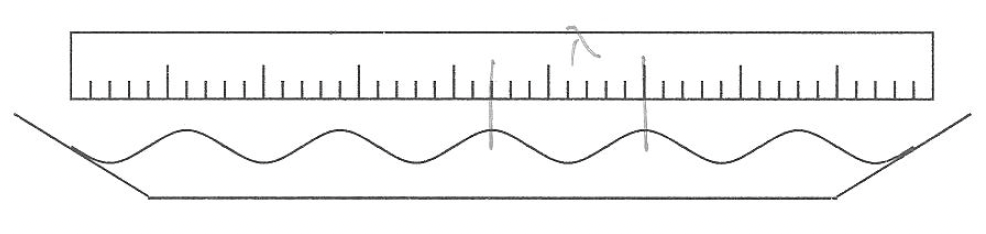
\includegraphics[width=0.75\linewidth]{images/Screenshot 2023-09-26 at 10.12.41 PM.png}


    \end{figure}

\end{frame}

\begin{frame}{量度水波的速率}
    \begin{itemize}
        \item 量度水波槽的兩點距離d。
        \item 使用直振源產生直線波的脈衝。
        \item 使用秒錶量度波傳播d的距離所需的時間t。
        \item 水波的速率\(v=\frac{d}{t}\)。
    \end{itemize}\bigskip

\end{frame}

\begin{frame}{水波槽}
    從牆壁反射的波可能會干擾到觀察的波紋。
    \begin{itemize}
        \item 為減少水波在牆內壁反射:
    \end{itemize}
    \begin{figure}
        \centering
        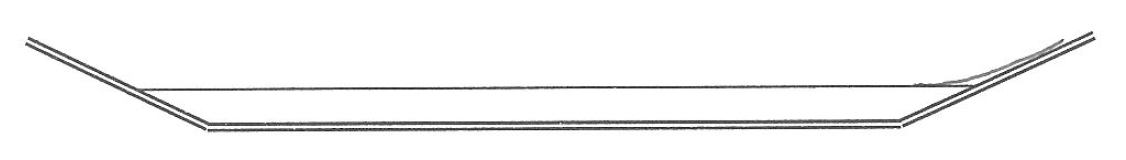
\includegraphics[width=0.75\linewidth]{images/Screenshot 2023-09-26 at 10.23.04 PM.png}
        \caption{四邊傾斜}

    \end{figure}
    \begin{figure}
        \centering
        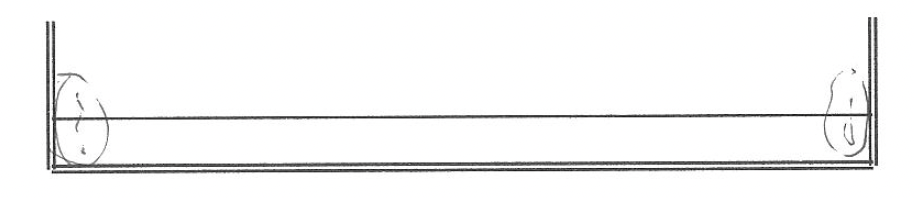
\includegraphics[width=0.7\linewidth]{images/Screenshot 2023-09-26 at 10.23.08 PM.png}
        \caption{內壁鋪上海綿}

    \end{figure}
\end{frame}

\begin{frame}{例題}
    增加直振源或點振源的振動頻率,對直線波或圓形波會有甚麼影響?

    \bigskip
    \begin{itemize}
        \item 水深不變,波速也不變。
        \item 根據公式 \(v=f\lambda\)\ $\Rightarrow$頻率 $\uparrow$,波長 $\downarrow$。
    \end{itemize}

\end{frame}


\begin{frame}{反射}
    \begin{figure}
        \centering
        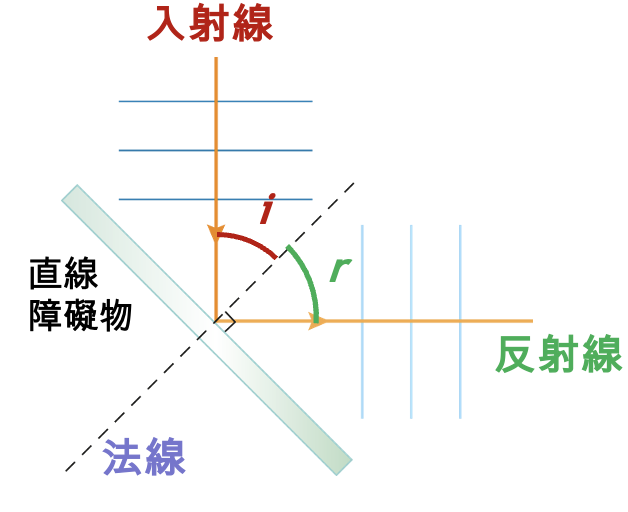
\includegraphics[width=0.5\linewidth]{images/Screenshot 2023-09-26 at 11.31.26 PM.png}


    \end{figure}
    \begin{itemize}
        \item 法線:垂直於反射面的虛構直線
        \item 入射角 i:入射線和法線之間的夾角
        \item 反射角 r:反射線和法線之間的夾角
    \end{itemize}
\end{frame}

\begin{frame}{波的反射現象}
    \begin{exampleblock}{反射定律}

        反射角 r = 入射角 i
    \end{exampleblock}
    \begin{itemize}
        \item 反射發生在障礙物或邊界。
        \item 反射的過程中
              \begin{itemize}
                  \item 速率、波長、頻率不變。
                  \item 波的相位可能改變。
                  \item 波的傳播方向必定改變。
              \end{itemize}
    \end{itemize}

\end{frame}


\begin{frame}{波的反射現象}
    \begin{figure}
        \centering
        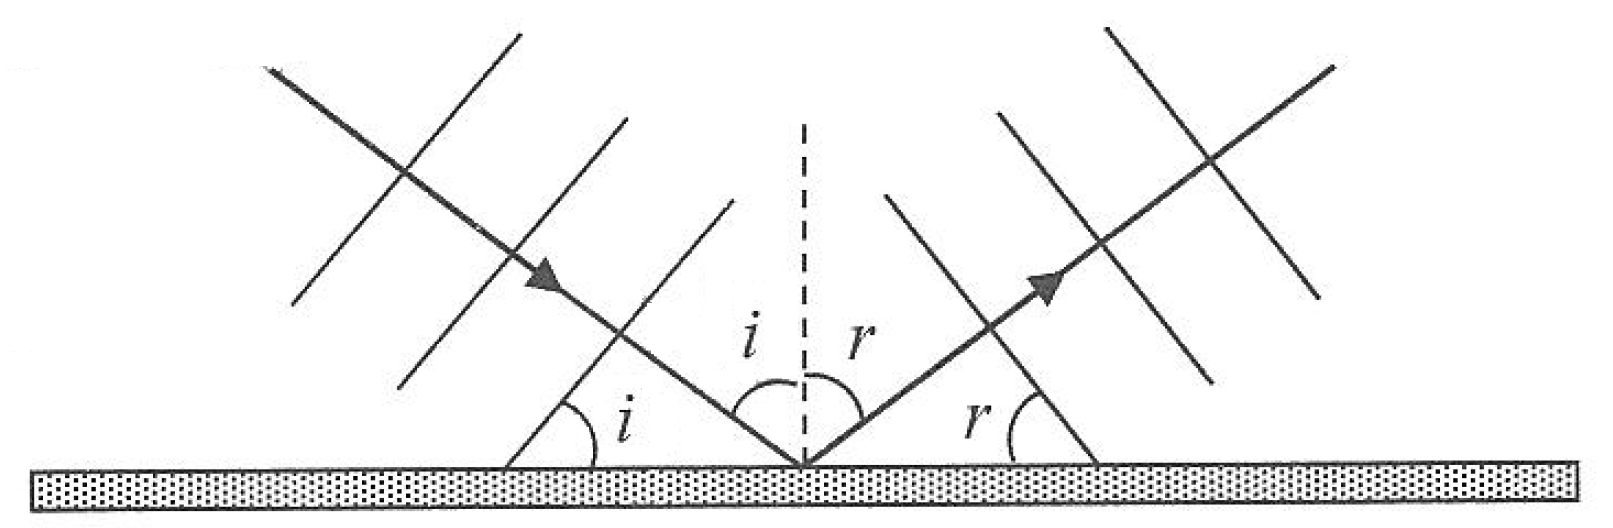
\includegraphics[width=0.5\linewidth]{images/Screenshot_21.png}
    \end{figure}\bigskip
    \begin{figure}
        \centering
        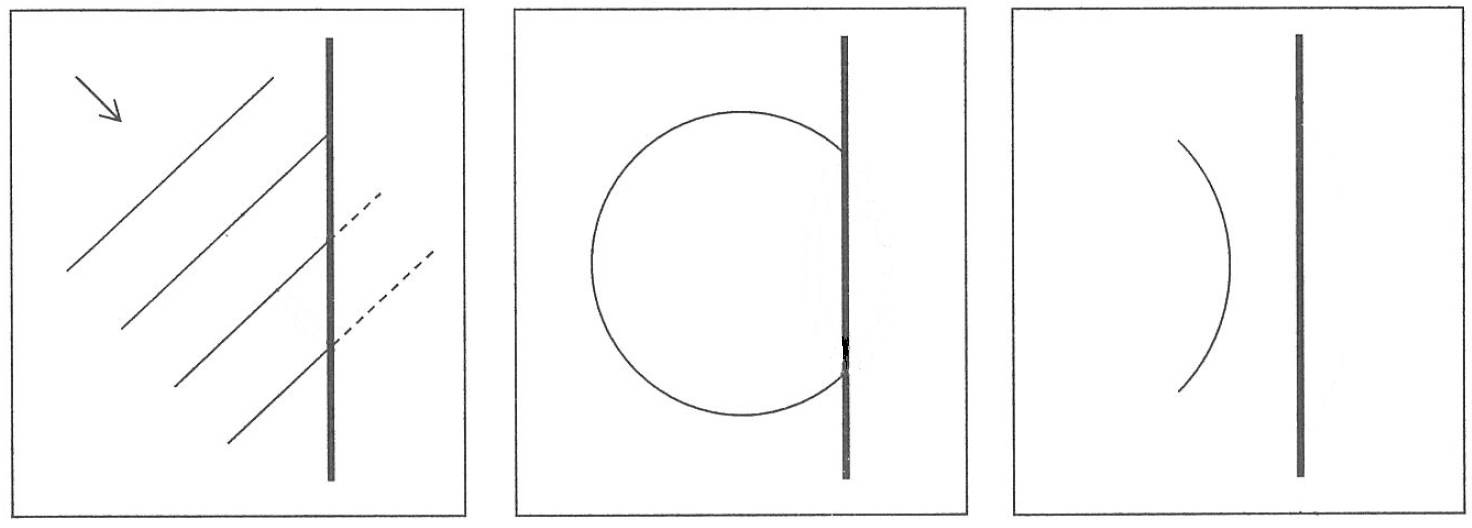
\includegraphics[width=1\linewidth]{images/Screenshot 2023-09-26 at 11.02.18 PM.png}
    \end{figure}
\end{frame}

\begin{frame}[t]{例題}
    \begin{figure}
        \centering
        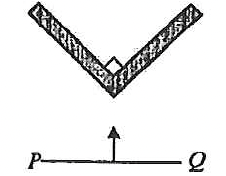
\includegraphics[width=0.25\linewidth]{images/Screenshot 2023-09-27 at 7.20.47 PM.png}


    \end{figure}
    畫出上圖可能的反射脈衝。
\end{frame}

\begin{frame}{例題}
    \begin{figure}
        \centering
        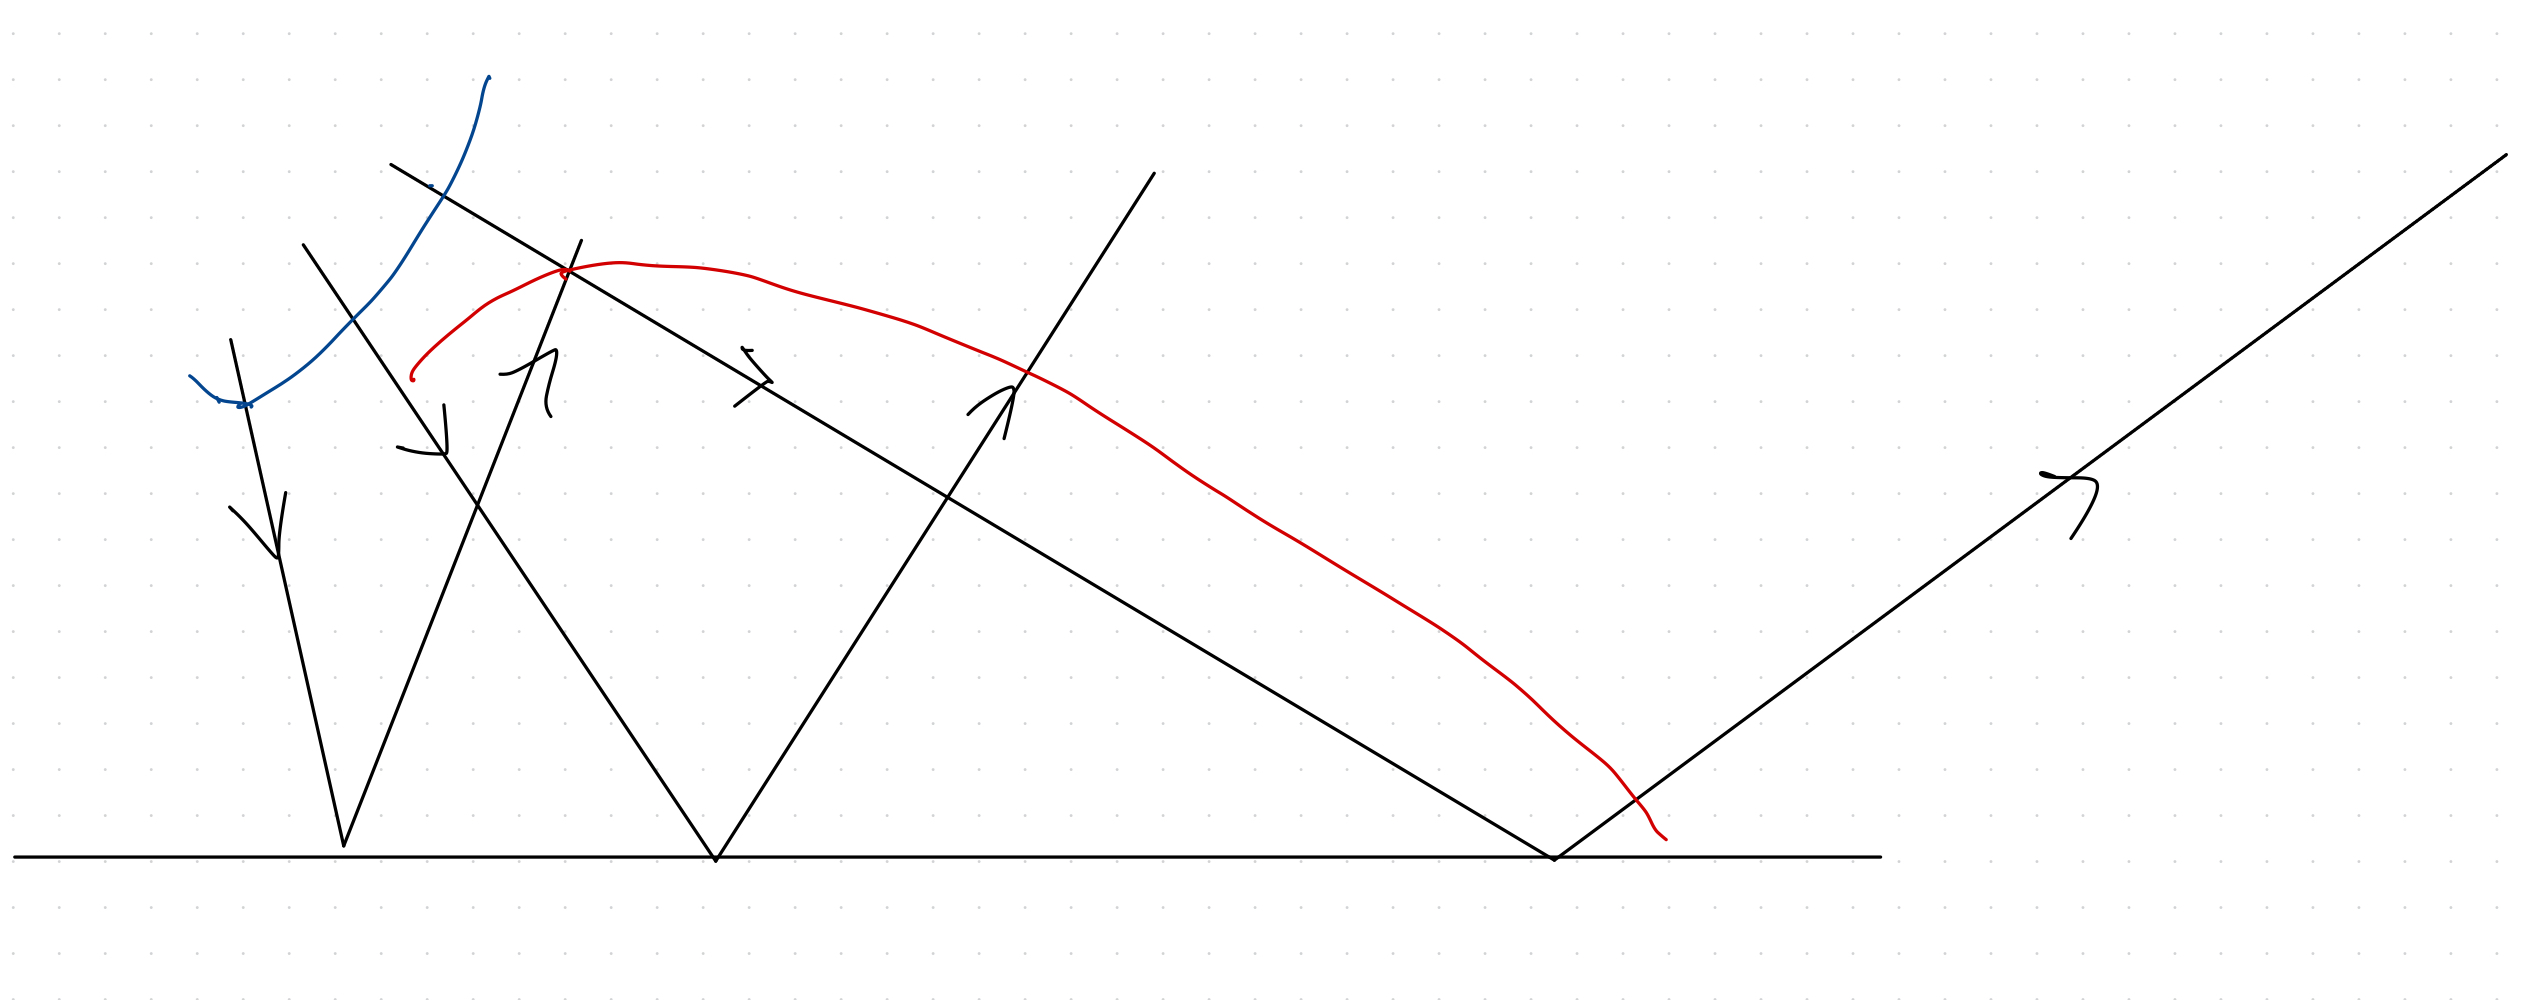
\includegraphics[width=1\linewidth]{images/IMG_F76D36A09E8B-1.jpeg}


    \end{figure}
\end{frame}

\begin{frame}{例題}
    \begin{columns}
        \column{.5\textwidth}
        \begin{figure}
            \centering
            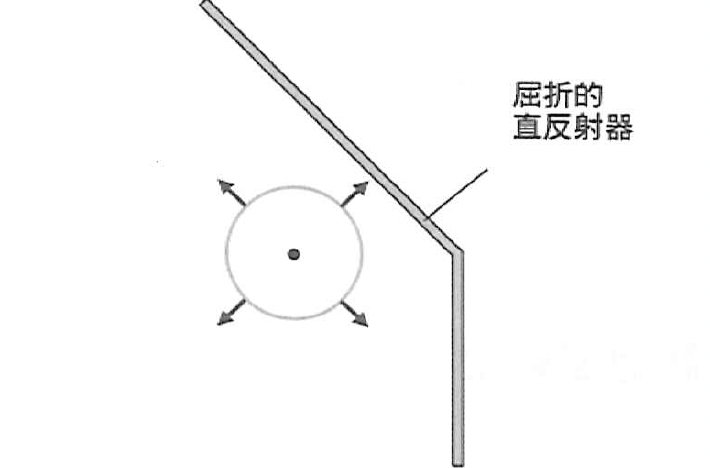
\includegraphics[width=1\linewidth]{images/Screenshot 2023-09-27 at 5.58.33 PM.png}
        \end{figure}
        \column{.5\textwidth}
        \begin{figure}
            \centering
            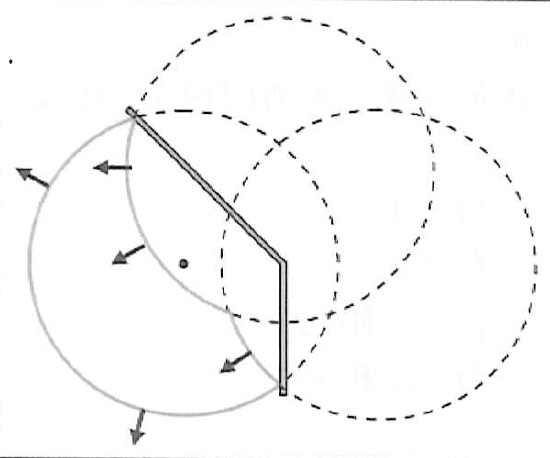
\includegraphics[width=1\linewidth]{images/Screenshot 2023-09-27 at 5.58.44 PM.png}
        \end{figure}
    \end{columns}


\end{frame}

\begin{frame}{例題}
    水波槽中有兩個相同的正方形方塊。方塊的角相互接觸,且均以一側沿南北方向擺放。一列直線波正以波陣面傾鈄 \qty{45}{^{\circ}} 的方向朝著方塊傳播,如圖所示。以下有關反射波的陳述,哪些是正確的?
    \begin{columns}
        \column{.5\textwidth}
        \begin{schoices}
            \item 部分反射波將沿原路折返。
            \item 部分反射波將沿正東方向傳播。
            \item 這列波將分為三部分,並以不同的方向傳播。
        \end{schoices}
        \column{.5\textwidth}
        \begin{figure}
            \centering
            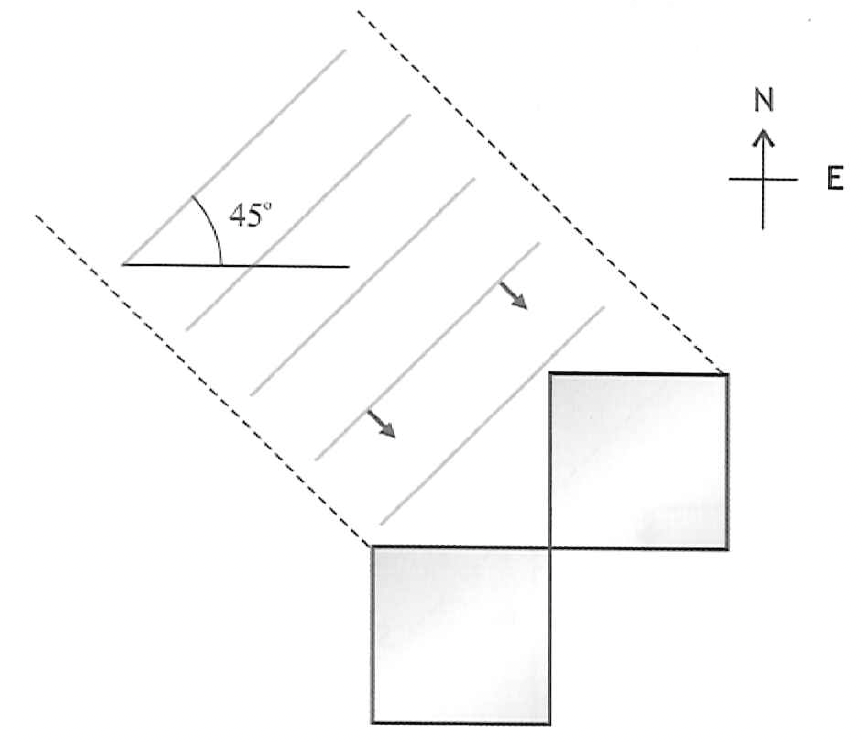
\includegraphics[width=0.7\linewidth]{images/Screenshot 2023-09-27 at 5.38.43 PM.png}


        \end{figure}
    \end{columns}

\end{frame}



\begin{frame}{例題}
    圖中顯示一個直線脈衝正朝著直角反射器傳播。下列哪些是正確的?

    \begin{figure}
        \centering
        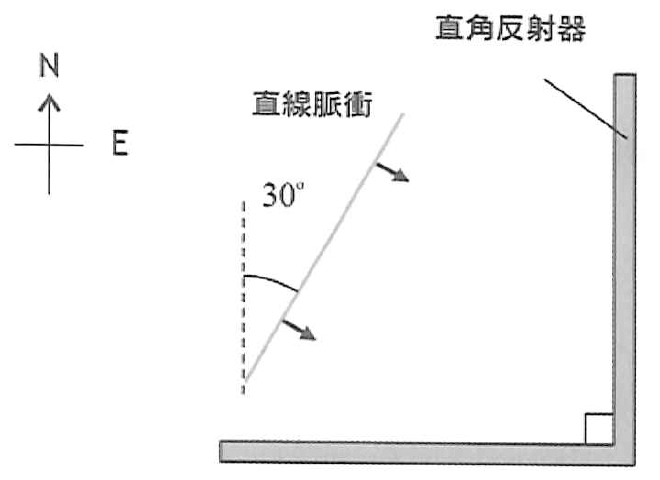
\includegraphics[width=0.4\linewidth]{images/Screenshot 2023-09-27 at 5.37.55 PM.png}
    \end{figure}
    \begin{mchoices}
        \item 反射的脈衝將分成兩部分,並以不同的方向離開。
        \item 這脈衝將受到反射器的兩面無止境重複的反射。
        \item 反射脈衝將沿原來的路徑離開反射器。
        \item 在反射過程中,脈衝經過\dg{60}角的旋轉。
    \end{mchoices}
\end{frame}

\begin{frame}{例題}
    一個圓形脈衝遇上直反射器,並已部分進行反射,哪個字母代表反射的部分?
    \begin{figure}
        \centering
        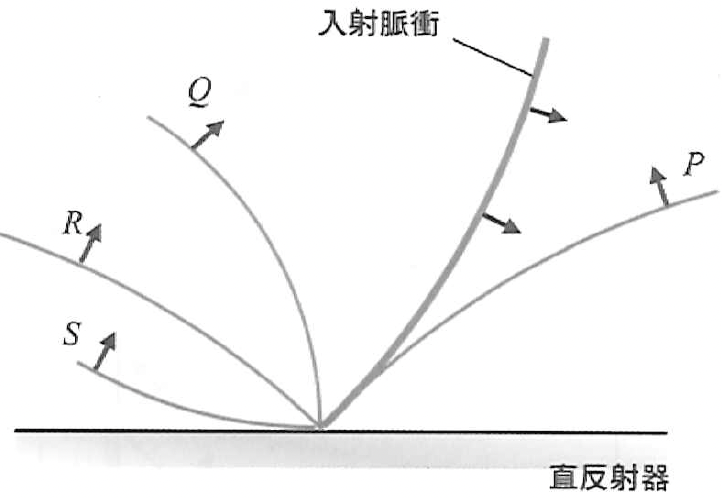
\includegraphics[width=0.5\linewidth]{images/Screenshot 2023-09-27 at 11.19.35 PM.png}


    \end{figure}
    \begin{mchoices}
        \begin{mmc}
            \item P
            \item Q
        \end{mmc}
        \begin{mmc}
            \item R
            \item S
        \end{mmc}
    \end{mchoices}
\end{frame}
\begin{frame}{測距儀}
    \begin{figure}
        \centering
        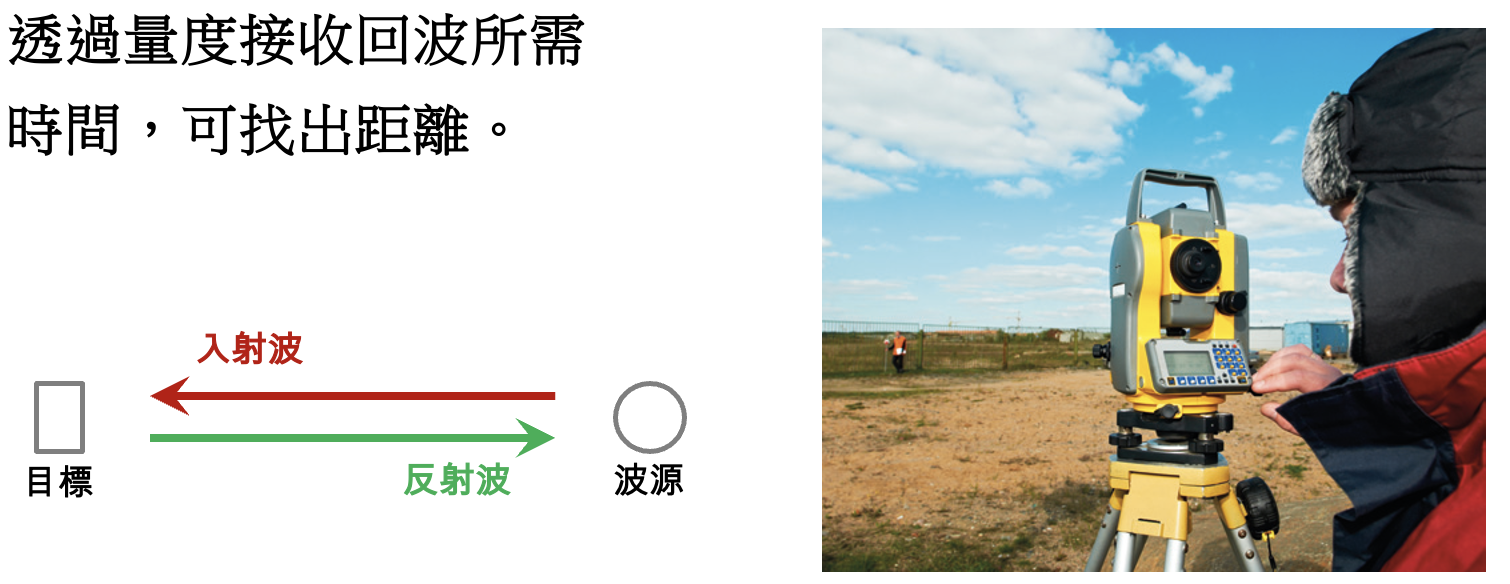
\includegraphics[width=1\linewidth]{images/Screenshot 2023-09-27 at 5.27.30 PM.png}


    \end{figure}
\end{frame}




\begin{frame}{反射和相位變化}
    \begin{itemize}
        \item 從繩子到牆壁,反射的波涉及$\pi(180^\circ)$相位改變。
    \end{itemize}\bigskip
    \begin{figure}
        \centering
        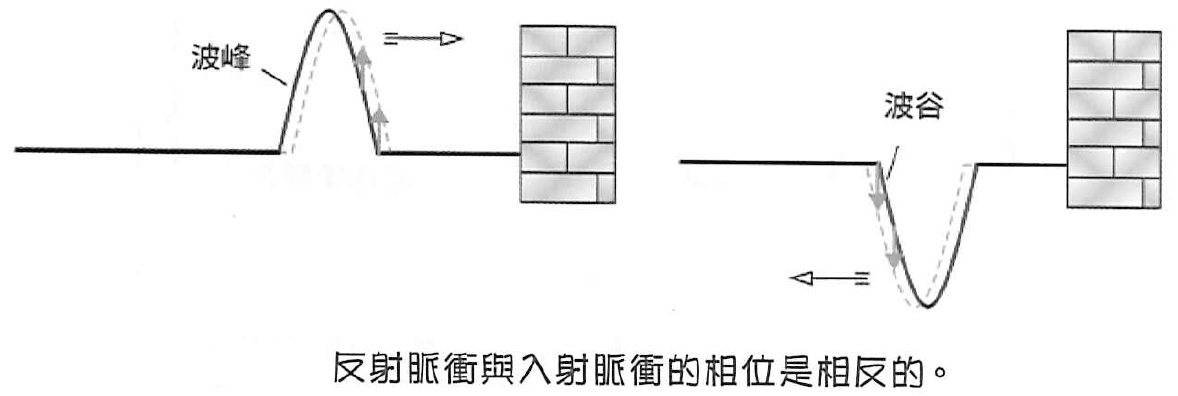
\includegraphics[width=\linewidth]{images/Screenshot 2023-09-27 at 7.11.55 PM.png}
        \label{fig:enter-label}
    \end{figure}
\end{frame}

\begin{frame}{反射和相位變化}
    \begin{itemize}
        \item 從繩子到自由端,反射的波相位沒有變化。
        \item 反射的\textbf{水波}在任何情況下都沒有相位變化。
    \end{itemize}\bigskip
    \begin{figure}
        \centering
        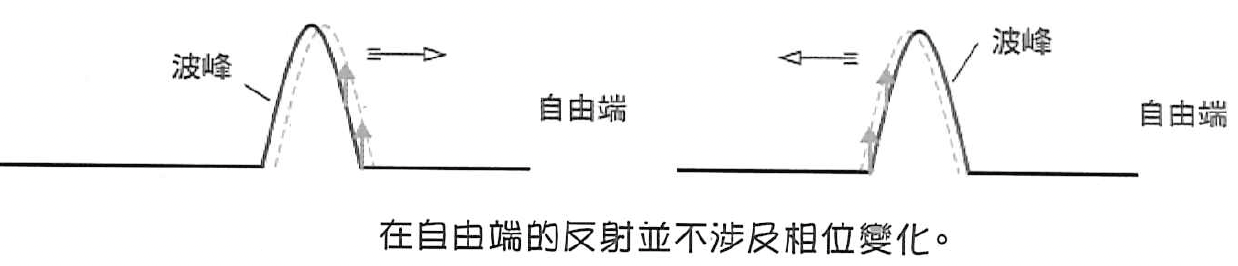
\includegraphics[width=1\linewidth]{images/Screenshot 2023-09-27 at 7.12.02 PM.png}


    \end{figure}

\end{frame}

\begin{frame}{反射和相位變化}
    \begin{figure}
        \centering
        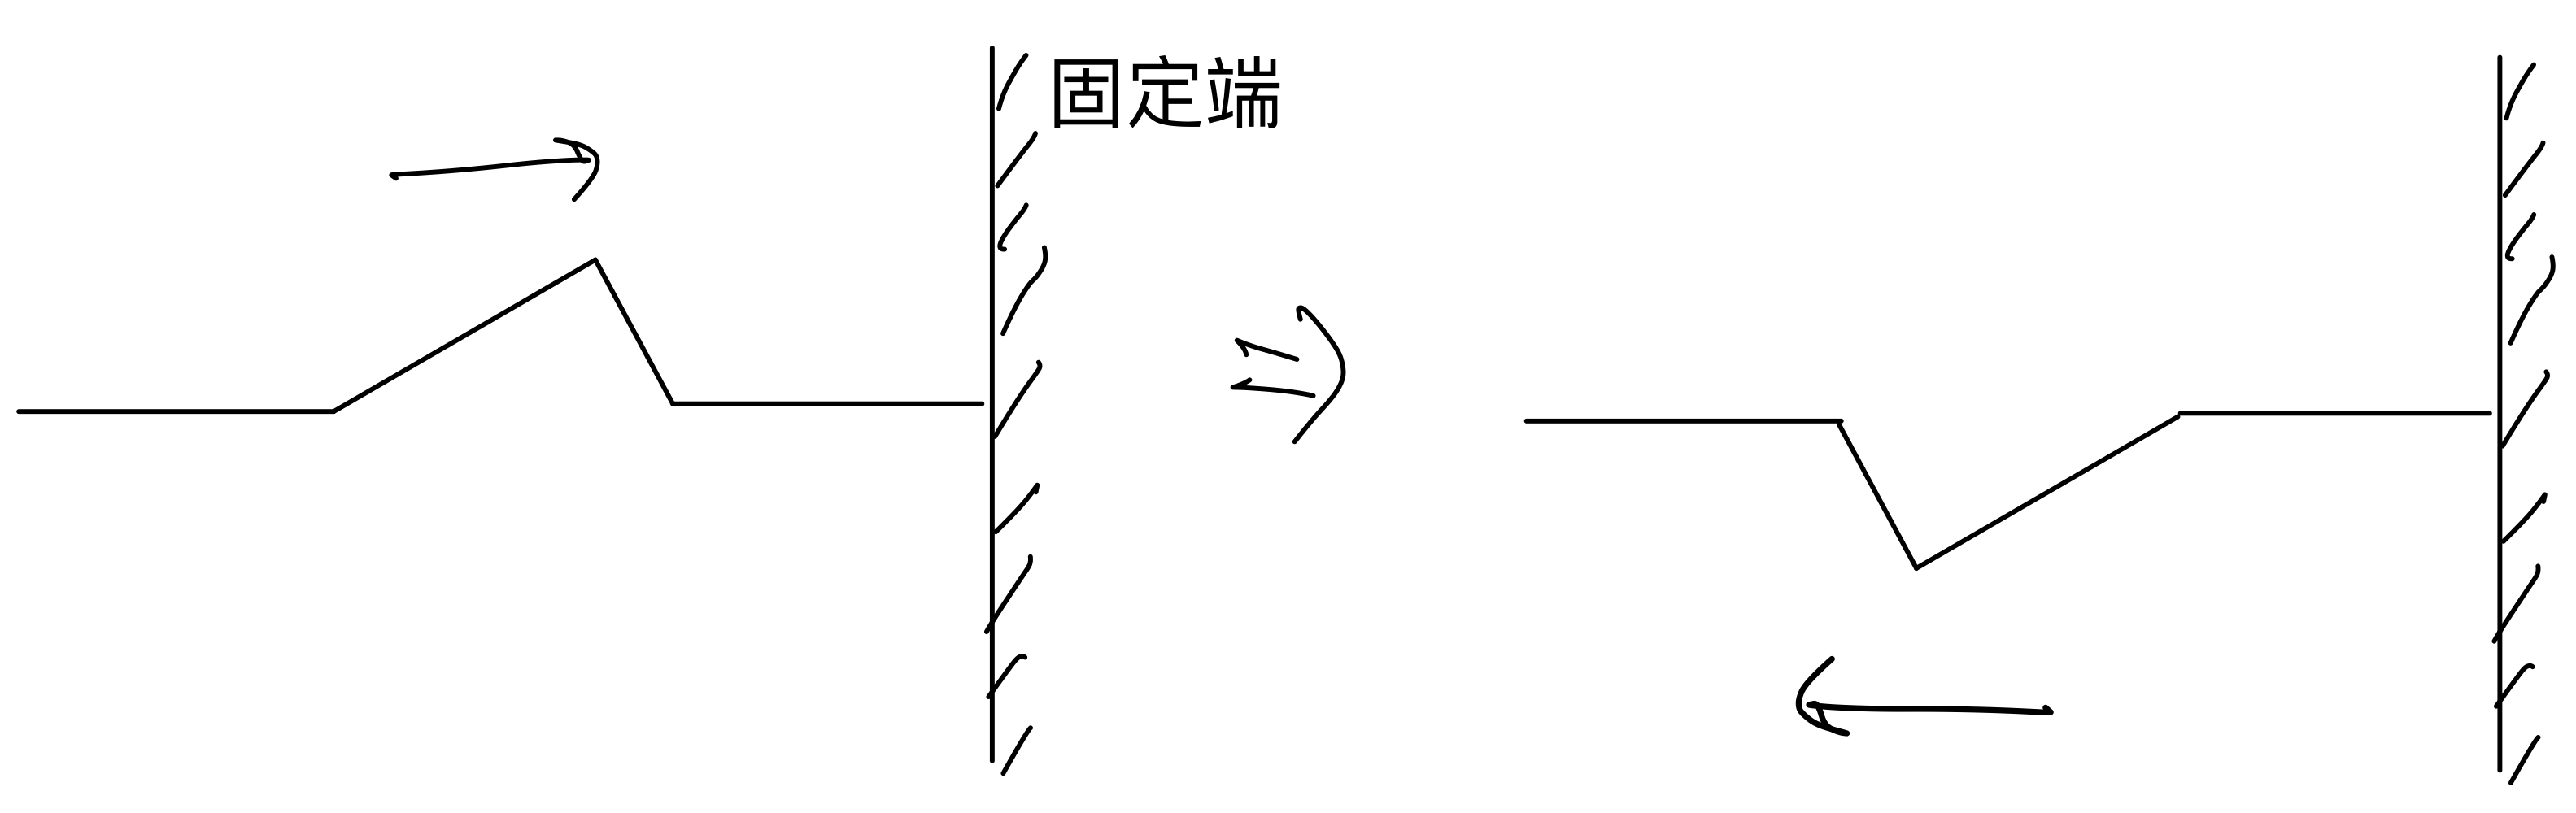
\includegraphics[width=0.75\linewidth]{images/IMG_6F6A16553544-1.jpeg}
        \caption{反射的波形上下左右倒轉}
    \end{figure}
    \begin{figure}
        \centering
        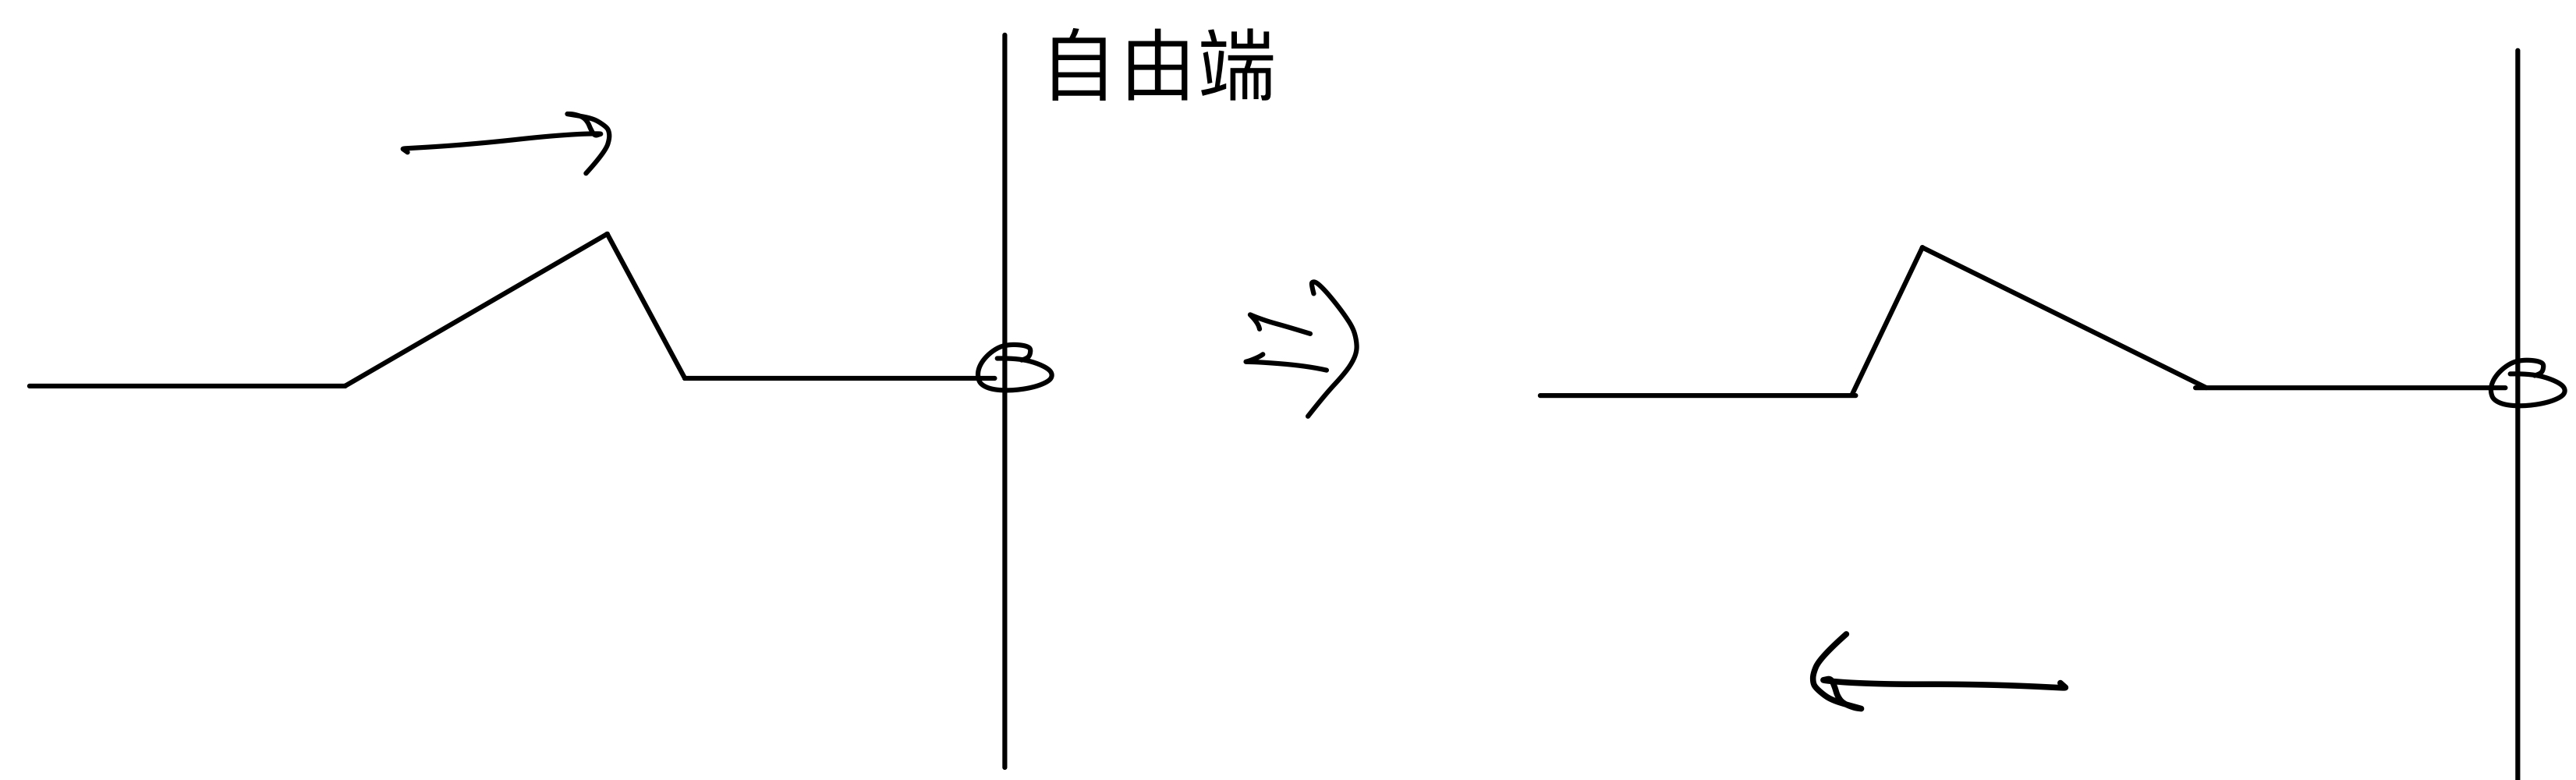
\includegraphics[width=0.75\linewidth]{images/IMG_CBCFA4B99FBF-1.jpeg}
        \caption{反射的波形上下倒轉}
    \end{figure}

\end{frame}



\begin{frame}{折射}
    折射是波動在兩種介質之間傳播時改變方向的現象。
    當波由一個介質進入另一個具有不同的介質時,便會發生折射。
    \begin{figure}
        \centering
        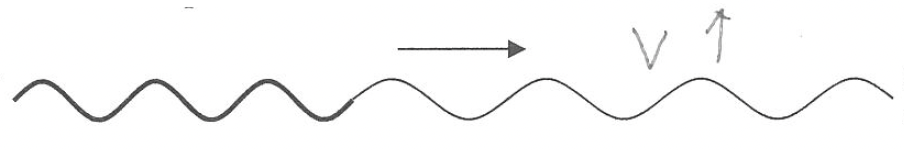
\includegraphics[width=0.75\linewidth]{images/Screenshot 2023-09-27 at 7.33.45 PM.png}
        \caption{左邊是粗繩,右邊是幼繩}

    \end{figure}
\end{frame}

\begin{frame}{折射}
    在折射的發生時,
    \begin{itemize}
        \item 頻率不變。
        \item 波速改變。
        \item 因為\(v=f\lambda\),波長必定改變。
        \item 如果是傾斜進入邊界,波的方向也會改變。
        \item 折射沒有相位改變。
    \end{itemize}
    \begin{figure}
        \centering
        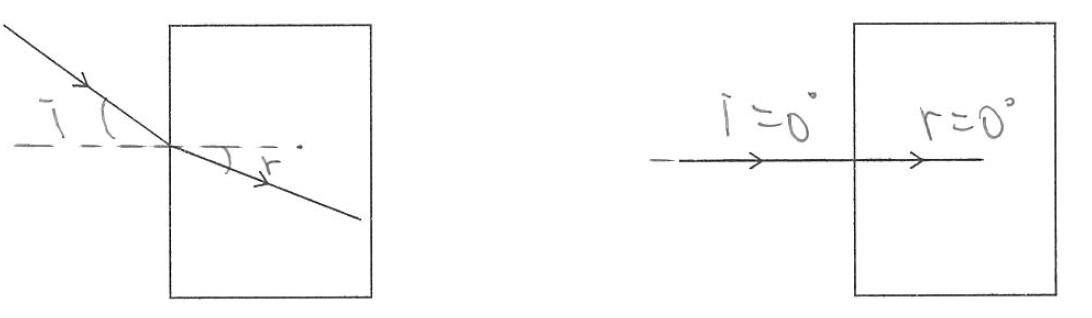
\includegraphics[width=0.75\linewidth]{images/Screenshot 2023-09-27 at 7.42.27 PM.png}
    \end{figure}
\end{frame}

\begin{frame}{折射}
    \begin{figure}
        \centering
        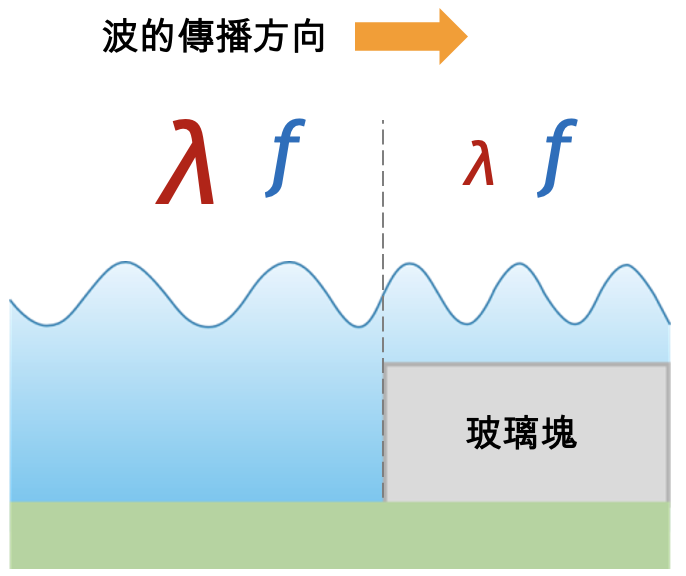
\includegraphics[width=0.7\linewidth]{images/Screenshot 2023-09-27 at 7.45.26 PM.png}
        \caption{深水快,淺水慢,$v\propto \lambda$}

    \end{figure}
\end{frame}

\begin{frame}{一個非波例子}
    \begin{figure}
        \centering
        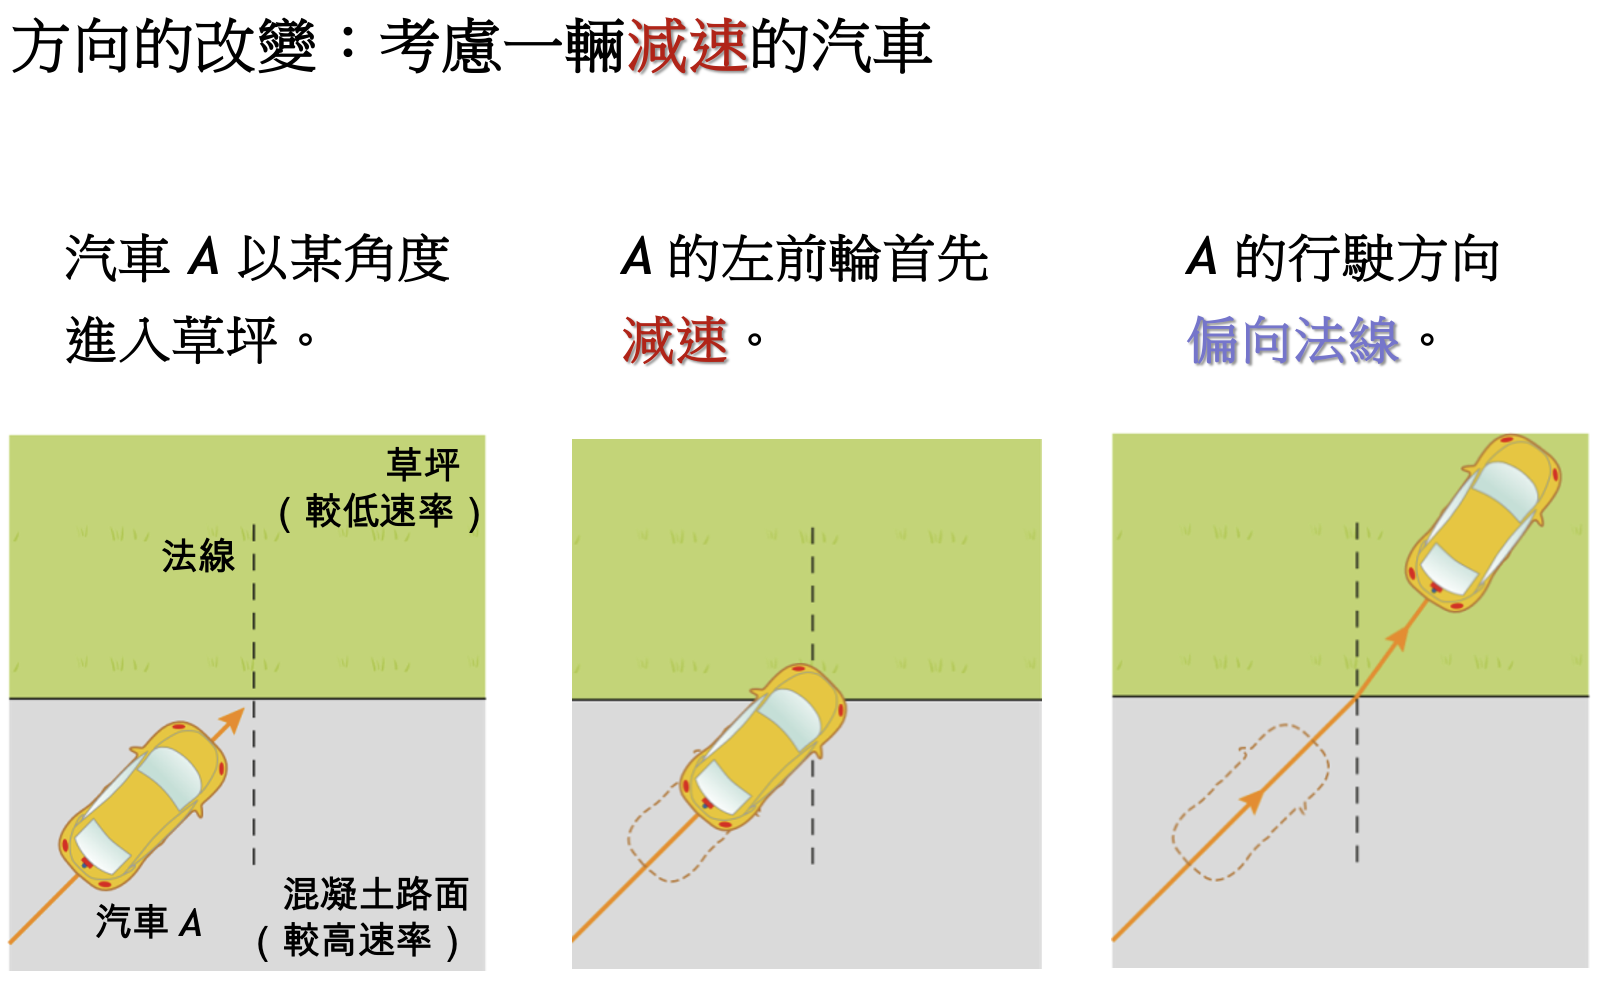
\includegraphics[width=1\linewidth]{images/Screenshot 2023-09-27 at 9.43.07 PM.png}


    \end{figure}
\end{frame}

\begin{frame}{一個非波例子}
    \begin{figure}
        \centering
        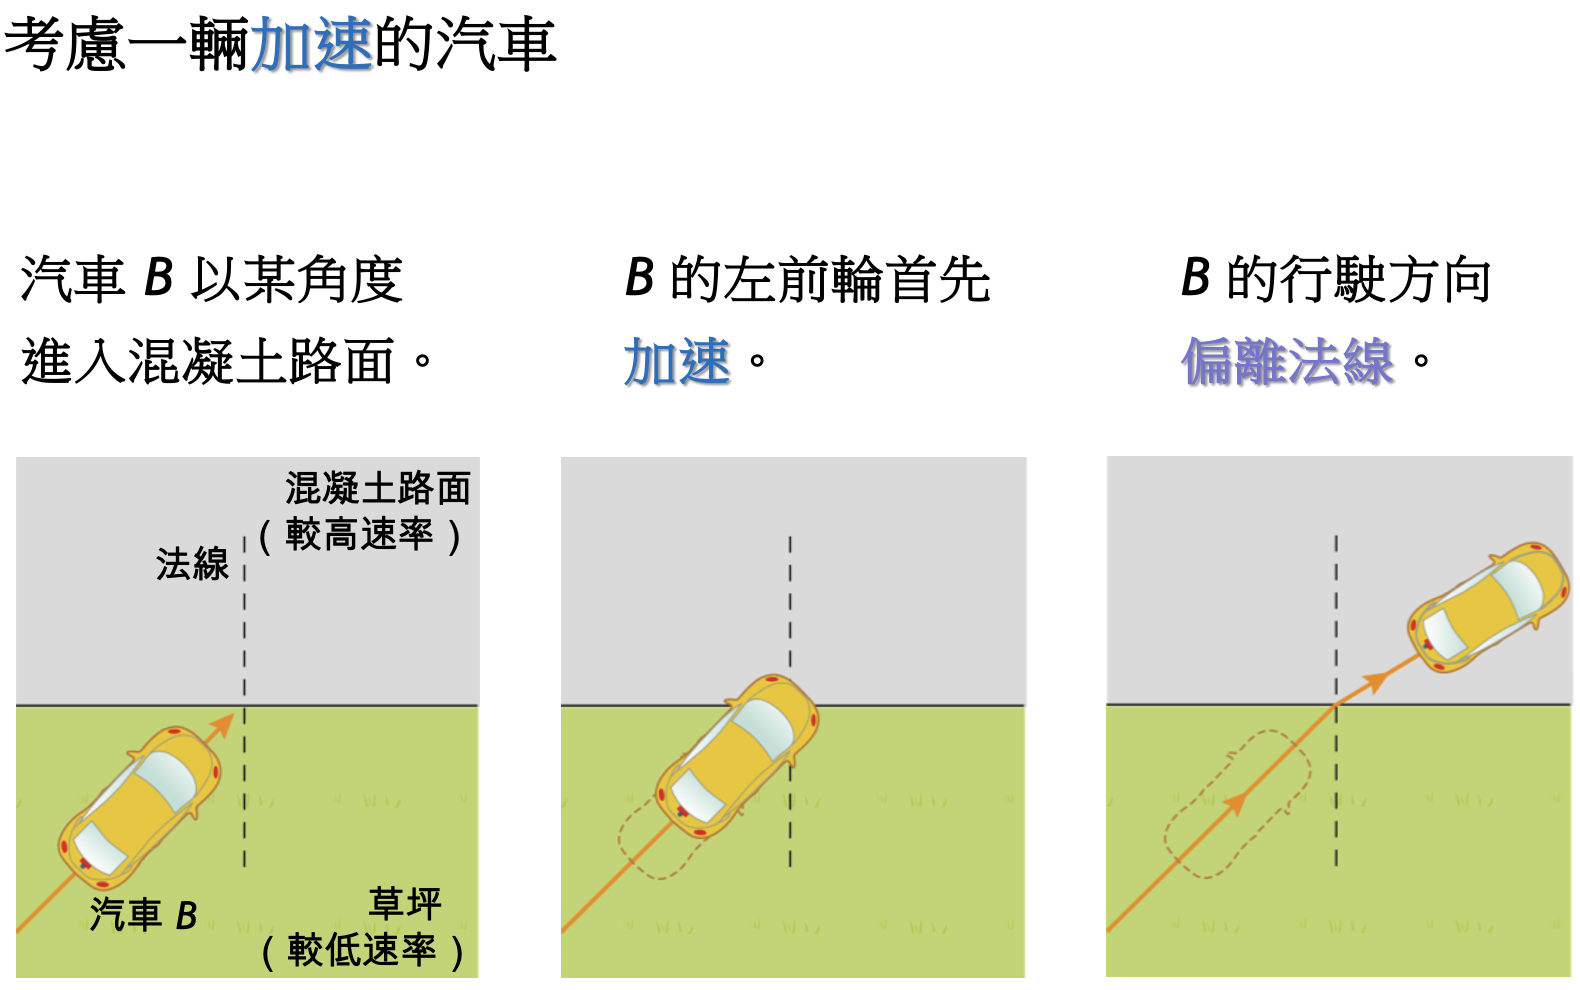
\includegraphics[width=1\linewidth]{images/Screenshot 2023-09-27 at 9.43.15 PM.png}


    \end{figure}
\end{frame}

\begin{frame}{折射波的方向改變}
    \begin{figure}
        \centering
        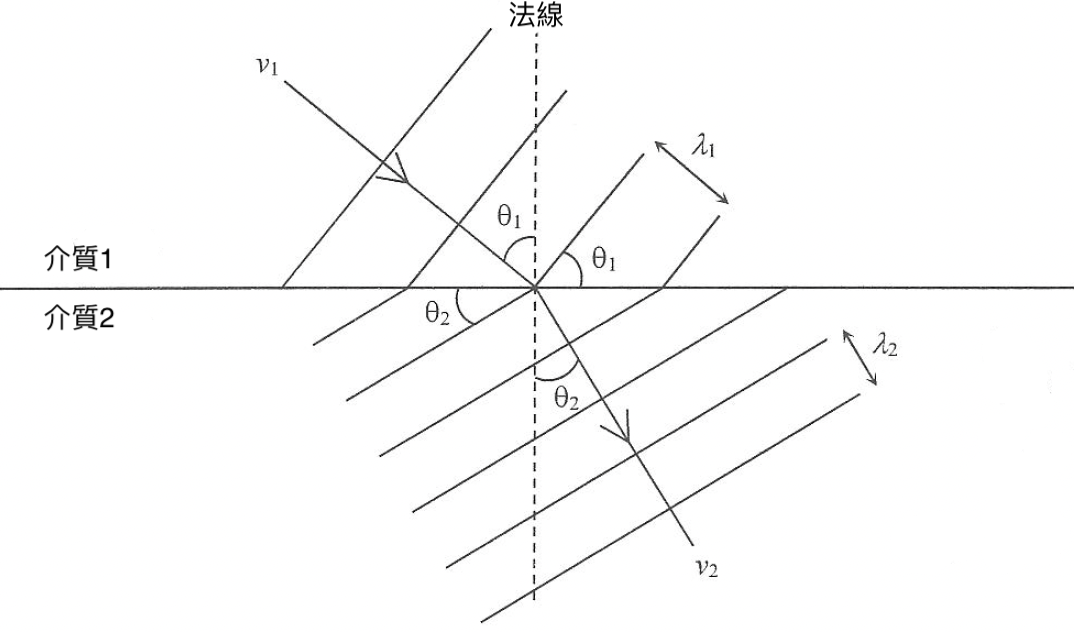
\includegraphics[width=0.6\linewidth]{images/Screenshot 2023-09-27 at 7.58.53 PM.png}
    \end{figure}
    \begin{alertblock}{波的折射定律}
        \[\frac{\sin \theta_1}{\sin\theta_2}=\frac{v_1}{v_2}=\frac{\lambda_1}{\lambda_2}\]
    \end{alertblock}
\end{frame}
\begin{frame}{折射波的方向改變}
    \begin{columns}
        \column{.5\textwidth}
        \begin{figure}
            \centering
            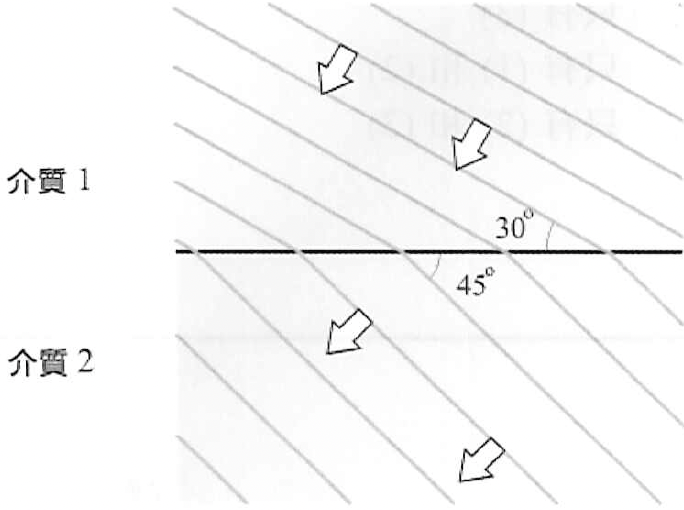
\includegraphics[width=\linewidth]{images/Screenshot 2023-09-27 at 8.51.39 PM.png}


        \end{figure}
        \column{.5\textwidth}
        \begin{figure}
            \centering
            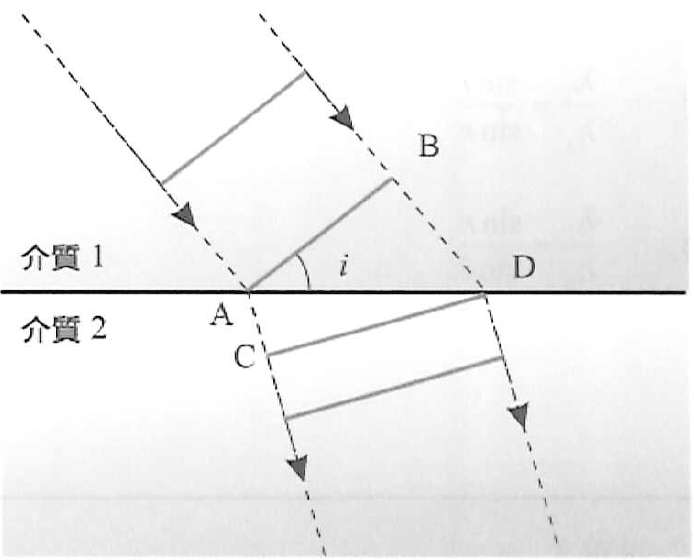
\includegraphics[width=1\linewidth]{images/Screenshot 2023-09-27 at 8.47.44 PM.png}

        \end{figure}
    \end{columns}
    % \begin{figure}
    %     \centering
    %     \includegraphics[width=0.75\linewidth]{images/Screenshot 2023-09-27 at 8.51.39 PM.png}


    % \end{figure}
\end{frame}

\begin{frame}{水波在交界面上的折射}
    \begin{figure}
        \centering
        \includegraphics[width=1\linewidth]{images/Screenshot 2023-09-27 at 8.16.07 PM.png}


    \end{figure}
\end{frame}

\begin{frame}{水波在交界面上的折射}
    \begin{columns}
        \column{.5\textwidth}
        \begin{figure}
            \centering
            \includegraphics[width=1\linewidth]{images/Screenshot 2023-09-27 at 8.28.32 PM.png}


        \end{figure}
        \column{.5\textwidth}
        \begin{figure}
            \centering
            \includegraphics[width=1\linewidth]{images/Screenshot 2023-09-27 at 8.28.43 PM.png}


        \end{figure}
    \end{columns}
\end{frame}

\begin{frame}{水波在交界面上的折射}
    水波槽中央是一個平凸形狀的淺水區域:
    \begin{columns}
        \column{.5\textwidth}
        \begin{figure}
            \centering
            \includegraphics[width=1\linewidth]{images/Screenshot 2023-09-27 at 8.31.00 PM.png}


        \end{figure}
        \column{.5\textwidth}
        \begin{figure}
            \centering
            \includegraphics[width=1\linewidth]{images/Screenshot 2023-09-27 at 8.31.30 PM.png}


        \end{figure}
    \end{columns}
\end{frame}

\begin{frame}{水波在交界面上的折射}

    ...不同於反射,折射時波陣面不會出現「斷折」的情況。
    \begin{columns}
        \column{.5\textwidth}
        \begin{figure}
            \centering
            \includegraphics[width=1\linewidth]{images/Screenshot 2023-09-27 at 8.42.42 PM.png}


        \end{figure}
        \column{.5\textwidth}
        \begin{figure}
            \centering
            \includegraphics[width=1\linewidth]{images/Screenshot 2023-09-27 at 8.42.50 PM.png}


        \end{figure}
    \end{columns}
\end{frame}

\begin{frame}{For future reference...}

    從低速介質到高速介質,若入射角持續增加,最終會發生全內反射。
    \bigskip
    \begin{columns}
        \column{.5\textwidth}
        \begin{figure}
            \centering
            \includegraphics[width=1\linewidth]{images/Screenshot 2023-09-27 at 8.56.48 PM.png}


        \end{figure}
        \column{.5\textwidth}
        \begin{figure}
            \centering
            \includegraphics[width=1\linewidth]{images/Screenshot 2023-09-27 at 8.57.33 PM.png}


        \end{figure}
    \end{columns}
\end{frame}

\begin{frame}[t]{例題}
    試用折射的原理解釋為什麼海灘上的波浪總是平行於岸邊。\medskip
    \begin{itemize}
        \item 隨著水波接近岸邊,速率v逐漸減少。
        \item 行進方向持續彎曲朝向法線,直到與岸邊垂直。
        \item 所以波陣面平行於岸邊。
    \end{itemize}
    \bigskip
    \begin{columns}
        \column{.5\textwidth}
        \begin{figure}
            \centering
            \includegraphics[width=\linewidth]{images/Picture1.png}


        \end{figure}
        \column{.5\textwidth}
        \begin{figure}
            \centering
            \includegraphics[width=1\linewidth]{images/Picture2.png}


        \end{figure}
    \end{columns}
\end{frame}

\begin{frame}{當繩子遇上繩子(不考)}
    \begin{figure}
        \centering
        \includegraphics[width=0.85\linewidth]{images/Screenshot 2023-09-28 at 10.16.23 AM.png}
        \caption{波進入波密/波疏介質時,出現部分反射,部分折射的現象}

    \end{figure}
\end{frame}

\begin{frame}{衍射(繞射)}
    \begin{itemize}
        \item 當行波經過狹縫或阻礙物邊緣時,會發生衍射,擴散至狹縫或阻礙物後方的區域。
        \item 衍射時:
              \begin{itemize}
                  \item 速率、頻率和波長都不會改變。
                  \item 只會改變波在障礙物邊緣的傳播方向。
              \end{itemize}
        \item 衍射是波獨有的現象。可以用這現象來判斷一個事物是不是波。
    \end{itemize}
    \begin{figure}
        \centering
        \includegraphics[width=1\linewidth]{images/Screenshot 2023-09-27 at 9.46.49 PM.png}


    \end{figure}
\end{frame}

\begin{frame}{衍射}
    \begin{figure}
        \centering
        \includegraphics[width=1\linewidth]{images/Screenshot 2023-09-27 at 9.09.03 PM.png}


    \end{figure}
\end{frame}

\begin{frame}{影響衍射程度的因素}
    \begin{itemize}
        \item 衍射的程度是根據$\displaystyle \frac{\lambda}{\texttt{a}}$影響。
              \begin{itemize}
                  \item 波長$\uparrow\ \Rightarrow$衍射程度$\uparrow$
                  \item 狹縫寬度$\uparrow\ \Rightarrow$衍射程度$\downarrow$
              \end{itemize}
        \item 阻礙物的大小不影響衍射的程度,除非障礙物極小至能讓波直接穿過。
        \item 圓形波:\(\lambda \approx a\)
        \item 振幅減半:$\lambda \approx 2a$
    \end{itemize}
\end{frame}

\begin{frame}{不同縫隙寬度的衍射}
    \begin{figure}
        \centering
        \includegraphics[width=0.95\linewidth]{images/Screenshot 2023-09-27 at 9.51.08 PM.png}


    \end{figure}
\end{frame}

\begin{frame}{不同波長的衍射}
    \begin{figure}
        \centering
        \includegraphics[width=0.95\linewidth]{images/Screenshot 2023-09-27 at 9.50.14 PM.png}


    \end{figure}
\end{frame}
\begin{frame}{例題}
    水波槽中,一道屏障中央有一個縫隙。以下哪些改變可增加平面水波穿過該縫隙時的繞射程度?
    \begin{schoices}
        \item 增加振動頻率。
        \item 減少水深。
        \item 減少縫隙的寬度。
    \end{schoices}
    \begin{mchoices}
        \begin{mmc}
            \item 只有(1)
            \item 只有(3)
        \end{mmc}
        \begin{mmc}
            \item 只有(1)和(2)
            \item 只有(2)和(3)
        \end{mmc}
    \end{mchoices}

    % \begin{mmchoices}
    %     \item 只有(1)
    %     \item 只有(3)
    %     \item 只有(1)和(2)
    %     \item 只有(2)和(3)
    % \end{mmchoices}
\end{frame}
\end{document}